\documentclass[aspectratio=169, dvipdfmx]{beamer}
\usetheme{Boadilla}
\usepackage{amsmath, amssymb, amsthm, color, latexsym}
\usefonttheme{professionalfonts}

\def\qed{\hfill $\Box$}
\def\endexample{\hfill $\clubsuit$}
\newcommand{\ex}{\mathbb{E}}
\newcommand{\var}{\mathrm{var}}
\newcommand{\bb}{\mathbb}
\newcommand{\cc}{\mathcal}

\title{3. Concentration of measure}
\author{Yoji Tomita}
\date{May 12, 2021}

\begin{document}

\maketitle

\begin{frame}{Introduction}
\begin{itemize}
    \item 2章を前提として, この章ではtail boundやconcentration inequalitiesを求めるためのより上級的な手法を紹介する.
    \item 3.1:Concentration by entropic techniques
    \item 3.2:A geometric perspective on concentration
    \item 3.3:Wasserstein distances and information inequalities
    \item 3.4:Tail bounds for empirical processes
\end{itemize}
\end{frame}

\section{3.1 Concentration by entropic techniques}

\begin{frame}{3.1 Concentration by entropic techniques}
\begin{itemize}
    \item エントロピーと, 集中不等式導出のためのその関連テクニックに関する議論から始める.
\end{itemize}
\end{frame}

\subsection{3.1.1 Entropy and its properties}
\begin{frame}{3.1.1 Entropy and its properties}
\begin{itemize}
    \item 凸関数 $\phi:\mathbb{R} \to \mathbb{R}$と, 確率変数$X\sim \mathbb{P}$に対して, $\phi$-entropyを
    \[\mathbb{H}_\phi(X) := \ex[\phi(X)] - \phi(\ex[X])\]
    とする($X, \phi(X)$の有限期待値は仮定).\\
     
    \item Jensenの不等式より, $\phi$-entropyは非負.
    \item これは$X$のばらつき加減を表す.
    \begin{itemize}
        \item 極端な場合, $X$がa.s.で期待値と一致するなら, $\mathbb{H}_\phi(X) = 0$.
    \end{itemize}
\end{itemize}
\end{frame}

\begin{frame}
\begin{itemize}
    \item 例1:$\phi(u) = u^2$なら$\mathbb{H}_\phi(X)$は分散.
        \[ \mathbb{H}_\phi(X) = \ex[X^2] - (\ex[X])^2 = \var(X).\]
     
    \item 例2:$\phi(u) = -\log u$, $Z := e^{\lambda X}$とすると,
        \[ \mathbb{H}_\phi(e^{\lambda X})  = -\lambda \ex[X] + \log \ex[e^{\lambda X}] = \log\ex[e^{\lambda(X-\ex[X])}]\]
        となり, centerd cumulant generating functionとなる.
\end{itemize}
\end{frame}

\begin{frame}
    \begin{itemize}
        \item この章では, 次の凸関数$\phi:[0,\infty)\to\mathbb{R}$に対するentropyを考える.
        \[\phi(u) := 
            \begin{cases}
                u\log u & \mathrm{for} \ u > 0\\
                0       & \mathrm{for} \ u = 0
            \end{cases}.\tag{3.1}\label{3.1}
        \]
        非負確率変数$Z$に対して, $\phi$-entropyは
        \[ \mathbb{H}(Z) = \ex[Z\log Z] - \ex[Z]\log\ex[Z], \tag{3.2}\label{3.2}\]
        となる(ただし関連する期待値の存在は仮定). 
        \begin{itemize}
            \item Shannon entropyやKullback-Leibler divergenceと関連がある(see Exercise 3.1).
            \item 以後このentropyを考えるので, $\mathbb{H}_\phi$のsubscrript $\phi$は省略.
        \end{itemize}
         
        \item $Z = e^{\lambda X}$とすると, $\mathbb{H}(e^{\lambda X})$は$X$のモーメント母関数$\varphi_X(\lambda)=\ex[e^{\lambda X}]$とその導関数$\varphi_X'(\lambda)$で表せる.
        \[\mathbb{H}(e^{\lambda X}) = \lambda \varphi_X'(\lambda) - \varphi_X(\lambda)\log\varphi_X(\lambda). \tag{3.3}\label{3.3}\]
    \end{itemize}
\end{frame}

\begin{frame}
\begin{exampleblock}{Example 3.1 (Entropy of a Gauusian random variable)}
    \begin{itemize}
        \item $X$は1次元正規分布$X\sim \mathcal{N}(0, \sigma^2)$とすると, $\varphi_X(\lambda) = e^{\lambda^2\sigma^2/2}, \varphi_X'(\lambda) = \lambda \sigma^2\varphi_X(\lambda)$なので,
        \[ \mathbb{H}(e^{\lambda X}) = \lambda^2\sigma^2\varphi_X(\lambda) - \frac{1}{2}\lambda^2\sigma^2\varphi_X(\lambda) = \frac{1}{2}\lambda^2\sigma^2\varphi_X(\lambda). \tag{3.4}\label{3.4}\]
    \end{itemize}
\end{exampleblock}
 \\
\begin{itemize}
    \item この節の残りで, このエントロピー(\ref{3.3})とtail boundsとの関連性を説明していく.
\end{itemize}
\end{frame}

\subsection{3.1.2 Herbst argument and its extensions}
\begin{frame}{3.1.2 Herbst argument and its extensions}
\begin{itemize}
    \item ある定数$\sigma > 0$が存在して, エントロピーが次の上限を満たすとする.
    \[ \mathbb{H}(e^{\lambda X}) \le \frac{1}{2}\sigma^2 \lambda^2\varphi_X(\lambda).\tag{3.5}\label{3.5} \]
    \begin{itemize}
        \item Example 3.1より, 正規分布$X\sim \mathcal{N}(0,\sigma^2)$は任意の$\lambda \in \mathbb{R}$に対し(3.5)をイコールで満たす.
        \item また任意のboundedな確率変数も(\ref{3.5})を満たす(Exercise 3.7).
    \end{itemize}
    \item このとき, その確率変数はsub-Gaussianとなる.
\end{itemize}
\begin{block}{Proposition 3.2 (Herbst argument)}
    エントロピー$\mathbb{H}(e^{\lambda X})$が(\ref{3.5})を任意の$\lambda \in I$ (ただし$I=[0, \infty)\ \mathrm{or}\ \mathbb{R}$)について満たすとする.
    このとき,
    \[ \log \ex[e^{\lambda(X-\ex[X])}] \le \frac{1}{2}\lambda^2\sigma^2 \ \ \ \mathrm{for\ all}\ \lambda\in I. \tag{3.6}\label{3.6} \]
\end{block}
\end{frame}

\begin{frame}{}
Remarks:
\begin{itemize}
    \item $I = \mathbb{R}$なら, (\ref{3.6})は$X-\ex[X]$がパラメータ$\sigma$のsub-Gauusianであることと同値.
    \item Chernoff argumentより, $I = [0, \infty)$で片側tail-bound
    \[ \mathbb{P}[X \ge \ex[X]+t] \le e^{-\frac{t^2}{2\sigma^2}} \tag{3.7}\label{3.7}\]
    が得られ, $I=\mathbb{R}$なら両側tail bounds
    \[ \mathbb{P}[|X-\ex[X]|\ge t] \le 2e^{-\frac{t^2}{2\sigma^2}}\]
    となる.
\end{itemize}
\end{frame}

\begin{frame}{}{} 
{\bf Proof.}
\begin{itemize}
    \item $I = [0,\infty)$の場合のみ示す($I=\mathbb{R}$は演習とする).
    \item エントロピーのモーメント母関数による表現(\ref{3.3})と仮定(\ref{3.5})より,
    \[\mathbb{H}(e^{\lambda X}) = \lambda \varphi'(\lambda) - \varphi(\lambda)\log\varphi(\lambda)\le\frac{1}{2}\sigma^2\lambda^2\varphi(\lambda) \ \ \ \forall \lambda \ge 0.\tag{3.8}\label{3.8} \]
    \item 関数$G$を$G(\lambda):= \frac{1}{\lambda}\log\varphi(\lambda)\ (\lambda\ne 0)$と定義し, $\lambda=0$では連続性を満たすように
    \[ G(0):= \lim_{\lambda \to 0}G(\lambda) = \ex[X] \tag{3.9}\label{3.9}\]
    とする.
    \item $G'(\lambda) = \frac{1}{\lambda}\frac{\varphi'(\lambda)}{\varphi(\lambda)}-\frac{1}{\lambda^2}\log\varphi(\lambda)$より, (\ref{3.8})は$G'(\lambda) \le \frac{1}{2}\sigma^2$となるので, $\lambda_0(>0)$から$\lambda$まで両辺積分すると
    \[ G(\lambda) - G(\lambda_0) \le \frac{1}{2}\sigma^2(\lambda-\lambda_0). \]
    \item $\lambda_0 \downarrow 0$とすると
    \[ G(\lambda) - \ex[X] \le \frac{1}{2}\sigma^2\lambda \]
    となり, これは(\ref{3.6})と同値である.\qed
\end{itemize}
\end{frame}

\begin{frame}{}
\begin{itemize}
    \item 2章と同様に, 次はsub-exponential tailをもつ確率変数を考える.
\end{itemize}
\begin{block}{Proposition 3.3 (Bernsten entropy bound)}
    正整数$b, \sigma$が存在して, エントロピー$\mathbb{H}(e^{\lambda X})$は以下を満たすとする.
    \[
        \mathbb{H}(e^{\lambda x})
        \le \lambda^2\left\{b\varphi_X'(\lambda) + \varphi_X(\lambda)(\sigma^2-b\ex[X])\right\}
        \ \ \ \mathrm{for\ all}\ \lambda \in [0, 1/b).
        \tag{3.10}\label{3.10}
    \]
    このとき, 
    \[
        \log\ex[e^{\lambda(X-\ex[X])}] \le \sigma^2\lambda^2(1-b\lambda)^{-1}
        \ \ \ \mathrm{for\ all}\ \lambda \in [0, 1/b).
        \tag{3.11}\label{3.11}
    \]
\end{block}
Remarks:
\begin{itemize}
    \item Chernoff argumentより, Prop.3.3は以下のsub-exponential tailsをもつ変数の上側Bernstein-type boundを含意する.
    \[
        \mathbb{P}[X\ge\ex[X] + \delta]
        \le \exp\left(-\frac{\delta^2}{4\sigma^2+2b\delta}\right)
        \ \ \ \mathrm{for\ all}\ \delta \ge 0.
        \tag{3.12}\label{3.12}
    \]
\end{itemize}
\end{frame}

\begin{frame}{}{}
{\bf Proof.}
\begin{itemize}
    \item 一般性を失わずに$\ex[X] = 0$と$b = 1$を仮定できる(see Exercise 3.6).
    \item このとき(\ref{3.10})は次のように簡単化される.
    \[
        \mathbb{H}(e^{\lambda X})
        \le \lambda^2 \left\{\varphi'(\lambda) + \varphi(\lambda)\sigma^2\right\}
        \ \ \ \mathrm{for\ all}\ \lambda \in [0,1).
        \tag{3.13}\label{3.13}
    \]
    \item Prop.3.2の証明と同様に$G(\lambda) = \frac{1}{\lambda}\log \varphi(\lambda)$を定義すると,
    (\ref{3.13})は$G' \le \sigma^2 + \frac{\varphi'}{\varphi}$と同値になる.
    \item $\lambda_0 > 0$を任意にとり$\lambda_0$から$\lambda$まで両辺積分すると,
    \[
        G(\lambda) - G(\lambda_0)
        \le \sigma^2(\lambda-\lambda_0) + \log\varphi(\lambda) - \log \varphi(\lambda_0).
    \]
    \item $\lambda_0 \downarrow 0$とすると,
    $\lim_{\lambda\downarrow 0}G(\lambda_0) = \ex[X]$と$\log\varphi(0)=0$より,
    \[
        G(\lambda) - \ex[X] \le \sigma^2 \lambda + \log\varphi(\lambda)
        \tag{3.14}\label{3.14}
    \]
    となる.
    \item (\ref{3.14})に$G$と$\varphi$を入れて書き換えると(\ref{3.11})が得られる.\qed
\end{itemize}
\end{frame}

\subsection{3.1.3 Separately convex functions and the entropic method}
\begin{frame}{3.1.3 Separately convex functions and the entropic method}
\begin{itemize}
    \item Entropy methodは複数の確率変数からなる関数のconcentrationを考える時に強力.
    \item 関数$f:\mathbb{R}^n \to \mathbb{R}$が{separately convex}であるとは,
          各$k\in\{1,\dots,n\}$について1変数関数
          \[y_k \mapsto f(x_1,\dots,x_{k-1},y_k,x_{k+1},\dots,x_n)\]
          が任意の$(x_1,\dots,x_{k-1},x_{k+1},\dots,x_n) \in \mathbb{R}^{n-1}$に対して凸であることをいう.
    \item また関数$f$がユークリッドノルムに対して$L$-Lipschitzであるとは,
          \[
              \left|f(x)-f(x')\right| \le L \|x-x'\|
              \ \ \ \mathrm{for\ all}\ x,x'\in\mathbb{R}^n.
          \]
          が成り立つことをいう.
\end{itemize}
\end{frame}

\begin{frame}
\begin{block}{Theorem 3.4}
    $\{X_i\}_{i=1}^n$は独立な確率変数列でそれぞれのサポートは$[a,b]$に含まれるものとし,
    $f:\mathbb{R}^n\to\mathbb{R}$はseparately convexかつ$L$-Lipschitzであるとする.
    このとき, 任意の$\delta > 0$に対して
    \[
        \mathbb{P}\left[ f(X) \le \ex[f(X)] + \delta \right]
        \le \exp\left(-\frac{\delta^2}{4L^2(b-a)^2}\right)
        \tag{3.16}\label{3.16}
    \]
    が成り立つ.
\end{block}
{Remarks:}
\begin{itemize}
    \item この結果はGaussianヘ変数のLipscitz関数のupper tail boundを求めたThm.2.26のanalogueだが,
          独立かつboundedな変数に対して適用できる.
    \item ただし, separetely convexityの仮定は一般に取り除くことができない.
    \item $f$がjointly convexの場合はlower tail boundの導出に他のテクニックが使える(cf Thm.3.24).
\end{itemize}
\end{frame}

\begin{frame}{}{}
{\bf Example 3.5} (Sharp bounds on Rademacher complexity)
    \begin{itemize}
        \item 有界部分集合$\mathcal{A}\in\mathbb{R}^n$は所与とし,
        確率変数$Z = \sup_{a\in\mathcal{A}}\sum_{k=1}^na_k\epsilon_k$を考える.
        \item $\epsilon_k \in \{ -1,1\}$はi.i.d.なRademacher variables.
        \item $Z$は線形関数の$\sup$をとったものなのでjointly (したがってseparately) convex.
        \item 別の$Z' = Z(\epsilon')$に対し, 任意の$a\in\mathcal{A}$について
        \[
            \langle a,\epsilon\rangle - Z'
            = \langle a,\epsilon\rangle - \sup_{a'\in\mathcal{A}}\langle a,\epsilon'\rangle
            \le \langle a, \epsilon-\epsilon'\rangle
            \le \|a\|_2 \|\epsilon-\epsilon'\|_2.
        \]
        \item $a\in \mathcal{A}$について$\sup$をとると
        $Z-Z' \le \sup_{a\in\mathcal{A}}\|a\|_2\|\epsilon-\epsilon'\|$.
        \item よって, $Z$は$\mathcal{W}(\mathcal{A}):=\sup_{a\in\mathcal{A}}\|a\|_2\|$-Lipschitz.
        \item したがって, Theorem 3.4より
        \[ \mathcal{P}[Z \le \ex[Z]+t] \le \exp\left(-\frac{t^2}{16\mathcal{W}^2(\mathcal{A})}\right).
        \tag{3.17}\label{3.17}\]
        \item 通常$\mathcal{W}^2(A)$は$\sum_{k=1}^n\sup a_k^2$よりずっと小さいので, Example2.25より強いboundとなる.
        \endexample
    \end{itemize}
\end{frame}

\begin{frame}{}{}
{\bf Example 3.6} (Operator norm of a random matrix)
\begin{itemize}
    \item $\mathbf{X} \in \mathbb{R}^{n^\times d}$はランダム行列で,
    $X_{ij}$は平均$0$, サポート$[-1,+1]$の分布からi.i.d.でひかれるとする.
    \item $|||\mathbf{X}|||_2$はスペクトルノルム(最大の特異値), or $\ell_2$-オペレータノルムとし, これは以下で与えられる.
    \[
        |||\mathbf{X}|||_{2}
        =\max _{v \in \mathbb{R}^{d} \atop \|v\|_{2}=1}\|\mathbf{X} v\|_{2}
        =\max _{v \in \mathbb{R}^{d}\atop \|v\|_{2}=1} \max _{u \in \mathbb{R}^{n} \atop\|u\|_{2}=1} u^{\mathrm{T}} \mathbf{X} v .
        \tag{3.18}\label{3.18}
    \]
    \item $\mathbf{X} \mapsto |||\mathbf{X}|||_2$を関数$f:\mathbb{R}^{nd}\to\mathbb{R}$と見ると,
    $f$はTheorem 3.4の仮定を満たす.
    \begin{itemize}
        \item $f$は線形な関数のsupremumなのでconvex,
        \item かつ
        \[
            \Big| |||\mathbf{X}|||_{2}-|||\mathbf{X}^{\prime}|||_{2}\Big|
            \stackrel{(\mathrm{i})}{\leq}|||\mathbf{X}-\mathbf{X}^{\prime}|||_{2}
            \stackrel{(\mathrm{ii})}{\leq}|||\mathbf{X}-\mathbf{X}^{\prime}|||_{\mathrm{F}},
            \tag{3.19}\label{3.19}
        \]
        となる($(\mathrm{i})$は三角不等式, $(\mathrm{ii})$はフロべニウスノルムは常にオペレータノルムを上からおさえることより)ので,
        $f$は$L=1$でLipschitz.
    \end{itemize}
    \item したがって, Theorem 3.4より,
    \[
        \mathbb{P}[|||\mathbf{X}|||_2\ge \ex[|||\mathbf{X}|||_2]+\delta]
        \le e^{-\frac{\delta^2}{16}}.
    \]
\end{itemize}
\end{frame}

\subsection{3.1.4 Tensorization and separately convex functions}
\begin{frame}{3.1.4 Tensorization and separately convex functions}
\begin{itemize}
    \item 2つのlemmaをもとにTheorem 3.4を証明する.
\end{itemize}
\begin{block}{Lemma 3.7}
    $X, Y \sim \mathbb{P}$, i.i.d.とすると, 任意の関数$g:\mathbb{R}\to\mathbb{R}$に対し以下が成り立つ.
    \[
        \mathbb{H}(e^{\lambda g(X)})
        \le \lambda^2\ex\left[(g(X)-g(Y))^2e^{\lambda g(X)}\mathbb{I}[g(X)\ge g(Y)]\right]
        \ \ \ \mathrm{for\ all}\ \lambda > 0.
        \tag{3.20a}\label{3.20a}
    \]
    さらに$X$のサポートが$[a,b]$に含まれ, $g$が凸かつLipschitzなら,
    \[
        \mathbb{H}(e^{\lambda g(X)})
        \le \lambda^2(b-a)^2\ex\left[(g'(X))^2e^{\lambda g(X)}\right]
        \ \ \ \mathrm{for\ all}\ \lambda>0,
        \tag{3.20b}\label{3.20b}
    \]
    が成り立つ($g'$は$g$の導関数).
\end{block}
\end{frame}

\begin{frame}{}
\begin{itemize}
    \item Lemma 3.7は, 凸かつLipschitzな関数はほとんどいたるところ微分可能であるという事実を使っている(Rademacher's Theorem).
    \item また, $g$が$L$-Lipschitzなら$\|g'\|_\infty \le L$\footnote{関数$f$に対して$\|f\|_\infty$は$f$の本質的上限$\|f\|_\infty:=\inf\{C\ge 0: |f(x)| \le C \mathrm{\ almost\ every}\ x.\}$.}なので,
          (\ref{3.20b})は以下を含意する.
          \[
              \mathbb{H}(e^{\lambda  g(X)}) \le \lambda^2 L^2(b-a)^2\ex[e^{\lambda g(X)}]
              \ \ \ \mathrm{for\ all}\ \lambda > 0.
          \] 
    \item したがってProposition 3.2より
    \[ \mathbb{P}[g(X) \ge \ex[g(X)]+\delta] \le e^{-\frac{\delta^2}{4L^2(b-a)^2}} \]
    となるので, Lemma 3.7はTheorem 3.4の1変数バージョンをただちに導く.
    \item しかし(\ref{3.20b})では$L$でなく$g'$とより強いboundとなっており,
    これがTheorem 3.4の導出において重要となる.
\end{itemize}
\end{frame}

\begin{frame}{}{}
{\bf Proof of Lemma 3.7}
\begin{itemize}
    \item エントロピーの定義より,
\begin{align*}
    \mathbb{H}(e^{\lambda g(X)})
    &= \ex_X[\lambda g(X) e^{\lambda g(X)}] - \ex_X[e^{\lambda g(X)}]\log(\ex_Y[e^{\lambda g(Y)}])\\
    &\le \ex_X[\lambda g(X) e^{\lambda g(X)}] - \ex_{X,Y}[e^{\lambda g(X)}\lambda g(Y)] \tag{Jensen's inequality}\\
    &= \frac{1}{2} \ex_{X,Y}\left[\lambda\{g(X)-g(Y)\}\{e^{\lambda g(X)}-e^{\lambda g(Y)}\}\right] \\
    &= \lambda \ex\left[\{g(X)-g(Y)\}\{e^{\lambda g(X)}-e^{\lambda g(Y)}\}\mathbb{I}[g(X) \ge g(Y)]\right]. \tag{3.22}\label{3.22}
\end{align*}
    となる(ただし最後の等式は$X,Y$の対称性より).
\end{itemize}
\end{frame}

\begin{frame}{}
\begin{itemize}
    \item 指数関数の凸性より, 任意の$s\ge t$に対し$e^s - e^t \le e^s(s-t)$なので,
    \[ (s-t)(e^s-e^t)\mathbb{I}[s\ge t] \le (s-t)^2e^s\mathbb{I}[s\ge t] \]
    \item これを(\ref{3.22})に適用すると, (\ref{3.20a})
    \[
        \mathbb{H}(e^{\lambda g(X)})
        \le \lambda^2\ex[(g(X)-g(Y))^2 e^{\lambda g(X)} \mathbb{I}[g(X)\ge g(Y)]].
        \tag{3.23}\label{3.23}
    \]
    が得られる.
    \item さらに$g$が凸で$x,y\in[a,b]$とすると, $g(x)-g(y)\le g'(x)(x-y)$より,
    \[(g(x)-g(y))^2\mathbb{I}[g(x)\ge g(y)] \le (g'(x))^2(x-y)^2\le (g'(x))^2(b-a)^2\]
    となるので, これを(\ref{3.23})に適用すれば(\ref{3.20a})が得られる.\qed
\end{itemize}
\end{frame}

\begin{frame}{}{}
{\bf Tensorization peoperty of entropy}
\begin{itemize}
    \item 関数$f:\mathbb{R}^n\to\mathbb{R}, k \in \{1,\dots,n\}, x_{\setminus k}=(x_i, i\ne k)\in\mathbb{R}^{n-1}$に対して,
    条件付きエントロピーを
    \[ \mathbb{H}(e^{\lambda f_k(X_k)} \mid x_{\setminus k}) := \mathbb{H}(e^{\lambda f(x_1,\dots,x_{k-1},X_k,x_{k+1},\dots,x_n)}) \]
    と定義する($f_k$は$x_k\mapsto f(x_1,\dots,x_k,\dots,x_n)$なる1変数関数).
    \item 確率変数$X^{\setminus k}\in \mathbb{R}^{n-1}$に対し,
    このエントロピー$\mathbb{H}(e^{\lambda f_k(X_k)} \mid X^{\setminus k})$は確率変数となる.
\end{itemize}
\begin{block}{Lemma 3.8 (Tensorization of entropy)}
$n$変数関数$f:\mathbb{R}^n \to \mathbb{R}$と, 独立な確率変数列$\{X_k\}_{k=1}^n$に対し,
\[
    \mathbb{H}(e^{\lambda f(X_1\dots,X_k)})
    \le \ex\left[ \sum_{k=1}^n\mathbb{H}(e^{\lambda f_k(X_k)} \mid X^{\setminus k}) \right]
    \ \ \ \mathrm{for\ all}\ \lambda > 0.
    \tag{3.21}\label{3.21}
\]
\end{block}
\end{frame}

\begin{frame}{}{}
{\bf Proof of Lemma 3.8}
\begin{itemize}
    \item まずエントロピーは以下のように表せる(Exercise 3.9).
    \[
        \mathbb{H}\left(e^{\lambda f(X)}\right)
        = \sup _{g}\left\{\mathbb{E}\left[g(X) e^{\lambda f(X)}\right] \mid \mathbb{E}\left[e^{g(X)}\right] \leq 1\right\}.
        \tag{3.24}\label{3.24}
        \]
    \item 各$j = 1,\dots,n$に対し, $X_j = (X_j\dots,X_n)$とする.
    \item $g$は$\ex[e^{g(X)}]\le 1$を満たす関数とする.
    \item 関数列$g_1,\dots, g_n$を以下で定義する.
    \begin{align*}
        &g^{1}\left(X_{1}, \ldots, X_{n}\right):=g(X)-\log \mathbb{E}\left[e^{g(X)} \mid X_{2}^{n}\right] \\
        &g^{k}\left(X_{k}, \ldots, X_{n}\right):=\log \frac{\mathbb{E}\left[e^{g(X)} \mid X_{k}^{n}\right]}{\mathbb{E}\left[e^{g(X)} \mid X_{k+1}^{n}\right]} \quad \mathrm{for}\ k=2, \ldots, n.
    \end{align*}
    \item すると定義より,
    \[
        \sum_{k=1}^{n} g^{k}\left(X_{k}, \ldots, X_{n}\right)=g(X)-\log \mathbb{E}\left[e^{g(X)}\right] \geq g(X).
        \tag{3.25}\label{3.25}
    \]
    で, さらに$\ex[\exp(g^k(X_k,\dots,X_n))\mid X_{k+1}^n] = 1$.
\end{itemize}
\end{frame}

\begin{frame}
\begin{itemize}
    \item このとき,
    \begin{align*}
        \mathbb{E}\left[g(X) e^{\lambda f(X)}\right] 
        & \stackrel{(\mathrm{i})}{\le} \sum_{k=1}^{n} \mathbb{E}\left[g^{k}\left(X_{k}, \ldots, X_{n}\right) e^{\lambda f(X)}\right] \\
        &=\sum_{k=1}^{n} \mathbb{E}_{X_{\setminus k}}\left[\mathbb{E}_{X_{k}}\left[g^{k}\left(X_{k}, \ldots, X_{n}\right) e^{\lambda f(X)} \mid X_{\backslash k}\right]\right] \\
        & \stackrel{(\mathrm{ii})}{\leq} \sum_{k=1}^{n} \mathbb{E}_{X_{\setminus k}}\left[\mathbb{H}\left(e^{\lambda f_{k}\left(X_{k}\right)} \mid X_{\backslash k}\right)\right]
    \end{align*}
    となる, ただし$(\mathrm{i})$は(\ref{3.25}), $(\mathrm{ii})$は(\ref{3.24})と$\ex[\exp(g^k(X_k,\dots,X_n))\mid X_{\backslash k}] = 1$より.
    \item これを関数$g \mathrm{\ s.t.\ } \ex[e^{g(X)}]\le 1$に対して$\sup$をとると, (\ref{3.24})より
    \[ \mathbb{H}(e^{\lambda f(X_1\dots,X_k)})
    \le \ex\left[ \sum_{k=1}^n \mathbb{H}(e^{\lambda f_k(X_k)} \mid X^{\setminus k}) \right] \]
    が得られる.\qed
\end{itemize}
\end{frame}

\begin{frame}{}{}
{\bf Proof of Theorem 3.4}
\begin{itemize}
    \item 各$k=1,\dots,n$と$x_{\backslash k}\in\mathbb{R}^{n-1}$について, 仮定より$f_k$は凸かつLipschitzなので,
    Lemma 3.7より 
    \begin{align*}
        \mathbb{H}\left(e^{\lambda f_{k}\left(X_{k}\right)} \mid x_{\backslash k}\right)
        &\leq \lambda^{2}(b-a)^{2} \mathbb{E}_{X_{k}}\left[\left(f_{k}^{\prime}\left(X_{k}\right)\right)^{2} e^{\lambda f_{k}\left(X_{k}\right)} \mid x_{\backslash k}\right] \\
        &=\lambda^{2}(b-a)^{2} \mathbb{E}_{X_{k}}\left[\left(\frac{\partial f\left(x_{1}, \ldots, X_{k}, \ldots, x_{n}\right)}{\partial x_{k}}\right)^{2} e^{\lambda f\left(x_{1}, \ldots, X_{k}, \ldots, x_{n}\right)}\right]
    \end{align*}
    \item Lemma 3.8より,
    \[
        \mathbb{H}\left(e^{\lambda f(X)}\right)
        \leq \lambda^{2}(b-a)^{2} \mathbb{E}\left[\sum_{k=1}^{n}\left(\frac{\partial f(X)}{\partial x_{k}}\right)^{2} e^{\lambda f(X)}\right]
        \stackrel{(\mathrm{i})}{\leq}  \lambda^{2}(b-a)^{2} L^{2} \mathbb{E}\left[e^{\lambda f(X)}\right]
    \]
    となる, ただし$\mathrm{(i)}$はLipschitz関数の性質
    $\|\nabla f(x)\|_{2}^{2}=\sum_{k=1}^{n}\left(\frac{\partial f(x)}{\partial x_{k}}\right)^{2} \leq L^{2}$
    より.
    \item したがって, Proposition 3.2を$f(X)$に適用すると, upper bound (\ref{3.16})が得られる.\qed
\end{itemize}
\end{frame}

\section{3.2 A geometric perspective on concentration}

\begin{frame}{3.2 A geometric perspective on concentration}
\begin{itemize}
    \item Concentration of measureの幾何的な面の議論に移る.
    \item この章の結果は, 距離測度空間(metric measure space)---つまり, 距離空間$(\mathcal{X}, \rho)$とそのボレル集合上の確率測度$\mathbb{P}$---の言葉で示される.
    \item 距離空間の例としては, 
    \begin{itemize}
        \item the Euclid space $\mathcal{X} = \mathbb{R}^n$ with the usual Euclidian metric $\rho(x,y):=\|x-y\|_2$,
        \item the discrete cube $\mathcal{X} = \{0, 1\}^n$ with the Hamming metric $\rho(x,y)=\sum_{j=1}^n\mathbb{I}[x_j\ne y_j]$
    \end{itemize}
    などがある.
\end{itemize}
\end{frame}

\subsection{3.2.1 Concentration functions}
\begin{frame}{3.2.1 Concentration functions}
\begin{itemize}
    \item 集合$A\subseteq \mathcal{X}$と点$x\in \mathcal{X}$に対し, それらの距離を以下とする.
    \[ \rho(x, A) := \inf_{y \in A}\rho(x, y). \tag{3.26}\label{3.26}\]
    \item パラメータ$\epsilon > 0$に対し, $A$の$\epsilon$-拡張($\epsilon$-enlargement)は以下で与えられる.
    \[ A^\epsilon := \{ x \in \mathcal{X} \mid \rho(x, A) < \epsilon \}. \tag{3.27}\label{3.27} \]
\end{itemize}
\begin{block}{Definition 3.9}
    距離測度空間$(\mathcal{X}, \rho, \mathbb{P})$のconcentration function $\alpha:[0,\infty)\to\mathbb{R}_+$は,
    \[
        \alpha_{\mathbb{P}, (\mathcal{X}, \rho)}(\epsilon)
        := \sup_{A \subseteq \mathcal{X}}\left\{ 1-\mathbb{P}[A^\epsilon]\ \Big|\ \mathbb{P}[A] \ge \frac{1}{2} \right\}
        \tag{3.28}\label{3.28}
    \]
    で定義される, ただし$\sup$は全ての可測部分集合$A$についてとられる.
\end{block}
\end{frame}

\begin{frame}{}{}
{\bf Example 3.10} (Concentration function for sphere)
\begin{itemize}
    \item $n$次元Euclidean sphere
    \[
        \mathbb{S}^{n-1} := \{x\in \mathbb{R}^n\mid \|x\|_2=1\}
        \tag{3.29}\label{3.29}
    \]
    上の一様分布$\mathbb{P}$と,
    geodesic distance $\rho(x, y):=\arccos\langle x,y\rangle$を考える.
    \item 各$y\in\mathbb{S}^{n-1}$に対し, hemisphere $H_y$ $(\mathbb{P}(H_y)=1/2)$を以下で定義する. (a)
    \[
        H_y
        := \{x\in \mathbb{S}^{n-1}\mid \rho(x,y) \ge \pi/2\}
        = \{ x \in \mathbb{S}^{n-1} \mid \langle x, y\rangle \le 0 \}.
        \tag{3.30}\label{3.30}
    \]
    \item この$\epsilon$-拡張は, 以下となる. (b)
    \[
        H_y^\epsilon = \{z\in \mathbb{S}^{n-1} \mid \langle z, y \rangle < \sin(\epsilon)\}.
        \tag{3.31}\label{3.31}
    \]
\end{itemize}
% \begin{center}
%     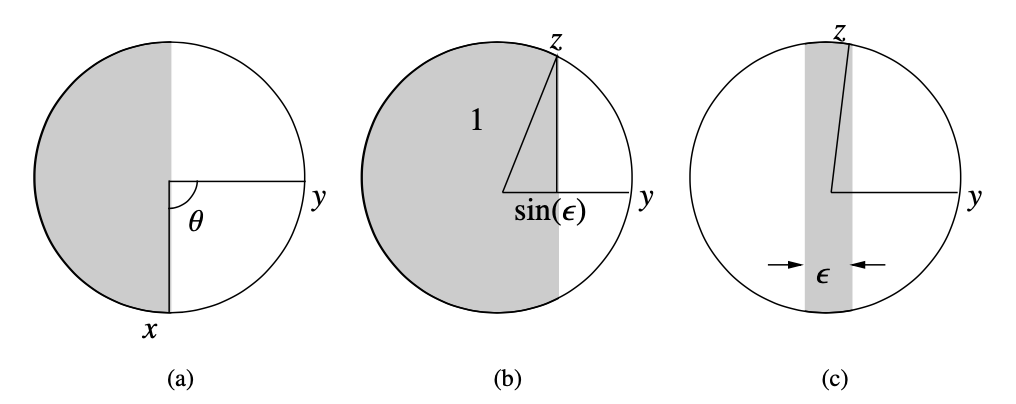
\includegraphics[width=8cm]{figure_3_1.png}
% \end{center}
\end{frame}

\begin{frame}{}{}
\begin{itemize}
    \item 一様分布であることより, concentration functionは, 
    \[
        \alpha_{\mathbb{S}^{n-1}}(\epsilon) = 1 - \mathbb{P}[H_y^\epsilon].
        \tag{3.32}\label{3.32}
    \]
    \item $\sin(\epsilon) \ge \epsilon/2$ (for all $\epsilon\in (0,\pi/2]$)より,
    $\mathbb{P}[H_y^\epsilon] \ge \mathbb{P}[\tilde{H}_y^\epsilon]$である, ただし
    \[
        \tilde{H}_y^\epsilon
        := \{z\in \mathbb{S}^{n-1} \mid \langle z, y\rangle \le \epsilon/2\}.
    \]
    \item さらに, 幾何的な計算により, 任意の$\epsilon \in (0, \sqrt{2})$に対して
    \[
        \mathbb{P}[\tilde{H}_y^\epsilon]
        \ge 1 - \left(1-\left(\frac{\epsilon}{2}\right)^2\right)^{n/2}
        \ge 1 - e^{-n\epsilon^2/8}
        \tag{3.33}\label{3.33}
    \]
    となる(?), ただし最後の不等号は$(1-t)\le e^{-t}$より.
    \item したがってconcentration functionの上限$\alpha_{\mathbb{S}^{n-1}}(\epsilon) \le e^{-n\epsilon^2/8}$が得られる.
    \item 似たアプローチでさらに注意深く上限をとると, より厳しい上限
    \[
        \alpha_{\mathbb{S}^{n-1}}(\epsilon) \le \sqrt{\frac{\pi}{2}}e^{-\frac{n\epsilon^2}{2}}
        \tag{3.34}\label{3.34}
    \]
    が得られる(?)
\end{itemize}
\end{frame}

\subsection{3.2.2 Connection to Lipschitz functions}
\begin{frame}{3.2.2 Connection to Lipschitz functions}
\begin{itemize}
    \item 関数$f:\mathcal{X}\to\mathbb{R}$が距離$\rho$に関して$L$-Lipschitzであるとは, 以下が成り立つことをいう.
    \[ |f(x)-f(y)| \le L \rho(x, y) \ \ \ \mathrm{for\ all}\ x,y\in\mathcal{X}. \tag{3.36}\label{3.36}\]
    \item 確率変数$X \sim \mathbb{P}$に対し, $m_f$は$f(X)$の任意のメディアンとする, つまり,
    \[ \mathbb{P}[f(X) \ge m_f] \ge 1/2\ \ \ \mathrm{and}\ \ \ \mathbb{P}[f(X) \le m_f] \ge 1/2. \tag{3.37}\label{3.37}\]
\end{itemize}
\begin{block}{Proposition 3.11}
\begin{itemize}
    \item 確率変数$X\sim \mathbb{P}$とconcentration function$\alpha_{\mathbb{P}}$に対し,
    $(\mathcal{X}, \rho)$上の$L$-Lipschitz関数$f$は次を満たす.
    \[ \mathbb{P}[|f(X)-m_f|\ge \epsilon] \le 2 \alpha_{\mathbb{P}}(\epsilon/L). \tag{3.39a}\label{3.39a}\]
    \item 関数$\beta:\mathbb{R}_+\to\mathbb{R}_+$は, 任意の$1$-Lipschitz関数$f$に対し
    \[ \mathbb{P}[f(X) \ge \ex[f(X)] + \epsilon] \le \beta(\epsilon)\ \ \ \mathrm{for\ any}\ \epsilon \ge 0. \tag{3.39b}\label{3.39b}\]
    を満たすとする. このとき, concentraion functionはbound $\alpha_{\mathbb{P}}(\epsilon) \le \beta(\frac{\epsilon}{2})$をもつ.
\end{itemize}
\end{block}
\end{frame}

\begin{frame}{}{}
{\bf Proof of Proposition 3.11}\\
{(前半)}
\begin{itemize}
    \item 集合$A = \{x\in\mathcal{X} \mid f(x) \le m_f\}$と, その$\epsilon/L$-拡張$A^{\epsilon/L}$について考える.
    \item 任意の$x \in A^{\epsilon/L}$に対し, $\rho(x, y) < \epsilon/L$なる$y\in A$が存在する.
    \item Lipschitz性より$|f(x) - f(y)| \le L\rho(x,y) < \epsilon$なので,
    \[ A^{\epsilon/L} \subseteq \{x\in\mathcal{X} \mid f(x) < m_f + \epsilon\}. \tag{3.38}\label{3.38} \]
    \item したがって,
    \[ 
        \mathbb{P}[f(X)\ge m_f+\epsilon]
        \stackrel{\mathrm{(i)}}{\le} 1-\mathbb{P}[A^{\epsilon/L}]
        \stackrel{\mathrm{(ii)}}{\le} \alpha_{\mathbb{P}}(\epsilon/L)
    \]
     が成り立つ, ただし$\mathrm{(i)}$は(\ref{3.38}), $\mathrm{(ii)}$は$\mathbb{P}(A) \ge 1/2$と$\alpha_{\mathbb{P}}$の定義より.
    \item 同様にして$\mathbb{P}[f(X)\le m_f-\epsilon] \le \alpha_{\mathbb{P}}(\epsilon/L)$も示されるので, (\ref{3.39a})が得られる.
\end{itemize}
\end{frame}

\begin{frame}{}{}
{(後半)}
\begin{itemize}
    \item $\epsilon \ge 0$を固定し, $A$は$\mathbb{P}[A]\ge 1/2$を満たす任意の可測集合とする.
    \item 関数$f(x) := \min\{\rho(x, A), \epsilon\}$は1-Lipschitz(らしい)で$1-\mathbb{P}[A^\epsilon]=\mathbb{P}[f(X)\ge\epsilon]$.
    \item また, 定義より$\ex[f(X)] \le (1-\mathbb{P}[A])\epsilon \le \epsilon/2$なので, 
    \[ \mathbb{P}\left[f(X)\ge \epsilon\right] \le \mathbb{P}\left[f(X)\ge\ex[f(X)]+\epsilon/2\right] \le \beta(\epsilon/2). \]
    \item したがって, 任意の可測集合$A \mathrm{\ s.t.\ }\mathbb{P}[A]\ge 1/2$に対して
    \[ 1-\mathbb{P}[A^\epsilon] \le \beta(\epsilon/2) \]
    となるので, $\alpha_{\mathbb{P}}(\epsilon) \le \beta({\epsilon/2})$.\qed
\end{itemize}
\end{frame}

\begin{frame}{}{}
{\bf Example 3.12} (L\'evy concentration on $\mathbb{S}^{n-1}$)
\begin{itemize}
    \item Example 3.10の$(\mathbb{S}^{n-1}, \rho, \mathbb{P})$において, concentration functionの上限は以下で得られた.
    \[
        \alpha_{\mathbb{S}^{n-1}}(\epsilon) \le \sqrt{\frac{\pi}{2}}e^{-\frac{n\epsilon^2}{2}}.
    \]
    \item したがって, 任意の$1$-Lipschitz関数$f:\mathbb{S}^{n-1}\to\mathbb{R}$に対して,
    \[
        \mathbb{P}[|f(X)-m_f| \ge \epsilon] \le \sqrt{2\pi}e^{-\frac{n\epsilon^2}{2}}
    \tag{3.40}\label{3.40}
    \]
    となる.
    \item さらに, Exercise 2.14(d)より, 以下も成り立つ.
    \[
        \mathbb{P}[|f(X) - \ex[f(X)]| \ge \epsilon] \le 2\sqrt{2\pi}e^{-\frac{n\epsilon^2}{8}}.
        \tag{3.41}\label{3.41}
    \]
    \endexample
\end{itemize}
\end{frame}

\begin{frame}{}{}
{\bf Example 3.13} (Concentration for Boolean hypercube)
\begin{itemize}
    \item Boolean hypercube $\mathcal{X} = \{0, 1\}^n$とHamming metric $\rho_H(x, y):= \sum_{j=1}^n\mathbb{I}[x_j\ne y_j]$を考える.
    \item 確率測度$\mathbb{P}$は$\mathcal{X}$上の一様分布.
    \item 半径$r$, 中心$x\in\mathcal{X}$の球をHamming ballと呼び, 以下で定義する.
    \[ \mathbb{B}_H(r; x) = \{y \in \{0,1\}^n \mid \rho_H(y,x)\le r\}. \]
    \item 非空な部分集合$A, B \subseteq \mathcal{X}$に対し, Harper's combinatorial theoremより,
    正整数$r_A, r_B$と対応する部分集合$A', B' \subseteq \mathcal{X}$が存在し, 以下を満たす.
    \begin{itemize}
        \item $\mathbb{B}_{H}\left(r_{A}-1 ; 0\right) \subseteq A^{\prime} \subseteq \mathbb{B}_{H}\left(r_{A} ; 0\right) \quad
            \mathrm{and} \quad \mathbb{B}_{H}\left(r_{B}-1 ; 1\right) \subseteq B^{\prime} \subseteq \mathbb{B}_{H}\left(r_{B} ; 1\right).$\footnote{$0,1$はそれぞれall-zeros vector, all-ones vector.}
        \item $\mathrm{card}(A) = \mathrm{card}(A'), \mathrm{card}(B)=\mathrm{card}(B')$.
        \item $\rho_H(A', B') \ge \rho_H(A, B)$.
    \end{itemize}
    \item 上の結果より, concentration functionは以下のように抑えられる.
    \[ \alpha_{\mathbb{P}}(\epsilon) \le \exp\left(-\frac{2\epsilon^2}{n}\right) \ \ \ \mathrm{for\ all}\ n\ge 3. \tag{3.42}\label{3.42} \]
\end{itemize}
\end{frame}

\begin{frame}
\begin{itemize}
    \item 任意の部分集合$A$ s.t. $\mathbb{P}[A] = \mathrm{card}(A)/2^n \ge 1/2$をとる.
    \item 任意の$\epsilon > 0$に対し, $B = \mathcal{X}\setminus A^\epsilon$とする.
    \item (\ref{3.42})にを示すには, $\mathbb{P}[B] \le \exp(-2\epsilon^2/n)$を示せば良い.
    \item $\epsilon \le 1$なら$\mathbb{P}[B]\le 1/2\le \exp(-2/n)\le \exp(-2\epsilon^2/n)$なので, 以後$\epsilon > 1$とする.
    \item 定義より,
    \[ \rho_H(A, B) = \min_{a \in A, b\in B}\rho(a,b) \ge \epsilon. \]
    \item $A', B'$をHarperの定理によって保証される集合とする. 
    \item $\mathrm{card}(A)=\mathrm{card}(A')\ge1/2$より, $A'$は$1$の数が$n/2$以下のベクトルを全て含む.
    \item $\rho_H(A', B')\ge \rho_H(A, B) \ge \epsilon$なので, $B'$は1の数が$n/2 + \epsilon$以上であるベクトルを全て含む.
\end{itemize}
\end{frame}

\begin{frame}
\begin{itemize}
    \item したがって, $\{X_i\}_{i=1}^n$をi.i.d. Bernoulli変数とすると, 上の議論とHoeffding boundより,
    \[\mathbb{P}[B]=\mathbb{P}[B']\le\mathbb{P}\left[\sum_{i=1}^nX_i\ge\frac{n}{2}+\epsilon\right] \le \exp\left(-\frac{2\epsilon^2}{n}\right)\]
    となり, $A$は$\mathbb{P}[A]\ge1/2$の任意の集合で$B = \mathcal{X}\setminus A^\epsilon$なので, (\ref{3.42})が得られる.
    \item よってProposition 3.11より, 任意の1-Lipschitz関数に対し
    \[ \mathbb{P}\left[\left|f(X)-m_{f}\right| \geq \epsilon\right] \leq 2 \exp\left(-\frac{2 \epsilon^{2}}{n}\right) .\]
    \endexample
\end{itemize}
\end{frame}

\subsection{3.2.3 From geometry to concentration}
\begin{frame}{3.2.3 From geometry to concentration}
\begin{itemize}
    \item これらの幾何的な面は, 凸幾何学とconcentration of measureの関連性を示唆する.
    \item たとえば, 次のBrunn-Minkowski inequalityを考えてみよう:
    \begin{itemize}
        \item $\mathrm{R}^n$上の任意の2つのcompact set $C, D \subset \mathbb{R}^n$に対し, 以下が成り立つ.
        {\footnotesize\[ \operatorname{vol}(\lambda C+(1-\lambda) D)
        \geq \left(\lambda\operatorname{vol}(C)^{1 / n}+(1-\lambda)\operatorname{vol}(D)^{1 / n}\right)^n
        \ge \operatorname{vol}(C)^\lambda \operatorname{vol}(D)^{1-\lambda}
         \quad \mathrm{for\ all}\ \lambda \in[0,1], \]}
         ただし, $\operatorname{vol}$はvolume, つまり$\mathrm{R}^n$上のLebesgue測度で, 
         \[\lambda C+(1-\lambda)D = \left\{\lambda c + (1-\lambda)d\mid c\in C,\ d\in D\right\}.\]
    \end{itemize}
    \item Concentration functionは$\mathbb{P}[A]\ge 1/2$のもとでの$1-\mathbb{P}[A^\epsilon]$の$\sup$だが,
    $\mathrm{vol}$を(正規化されていない)確率測度とみると, Brunn-Minkowski inequalityはこの上限の導出に使える.
\end{itemize}
\end{frame}

\begin{frame}{}{}
{\bf Example 3.14} (Classical isoperimetric inequality in $\mathbb{R}^n$)
\begin{itemize}
    \item $\mathbb{B}_2^n$を$\mathbb{R}^n$上のEuclidean sphereとする,
    つまり$\mathbb{B}_2^n:=\{x\in\mathbb{R}^n\mid \|x\|_2\le 1\}$.
    \item $A$は$\mathrm{vol}(A) = \mathrm{vol}(\mathbb{B}_2^n)$を満たす任意の集合$A\subset \mathbb{R}^n$とする.
    \item このとき, Brunn-Minkowski inequalityにおいて$\lambda, C, D$を適切に選ぶことで
    \[
        \left[\operatorname{vol}\left(A^{\epsilon}\right)\right]^{1 / n}
        =\left[\operatorname{vol}\left(A+\epsilon \mathbb{B}_{2}^{n}\right)\right]^{1 / n}
        \geq[\operatorname{vol}(A)]^{1 / n}+\left[\operatorname{vol}\left(\epsilon \mathbb{B}_{2}^{n}\right)\right]^{1 / n}
    \]
    となる(see Exercise 3.10).
    \item さらに, $\mathrm{vol}(A) = \mathrm{vol}(\mathbb{B}_2^n)$と$[\mathrm{vol}(\epsilon\mathbb{B}_2^n)]^{1/n} = \epsilon\mathrm{vol}(\mathbb{B}_2^n)^{1/n}$より\footnote{ここテキストでは$[\mathrm{vol}(\epsilon\mathbb{B}_2^n)]^{1/n} = \epsilon\mathrm{vol}(\mathbb{B}_2^n)$となっているがおそらくタイポ.},
    \[ 
        \mathrm{vol}(A^\epsilon)^{1/n}
        \ge (1+\epsilon) \mathrm{vol}(\mathbb{B}_2^n)^{1/n}
        = [\mathrm{vol}((\mathbb{B}_2^n)^\epsilon)]^{1/n}
    \]
    となるので, したがって
    \[
        \mathrm{vol}(A^\epsilon) \ge \mathrm{vol}([\mathbb{B}_2^n]^\epsilon).
        \tag{3.44}\label{3.44}
    \]
    \endexample
\end{itemize}
\end{frame}

\begin{frame}
    \begin{itemize}
        \item Brunn-Minkowski inequalityは, 次のfunctional-analytic generalizationが知られている.
    \end{itemize}
    \begin{block}{Theorem 3.15 (Pr\'ekopa-Leindler inequality)}
        $u,v,w$は非負可積分関数で, ある$\lambda \in [0, 1]$が存在して,
        \[ w(\lambda x + (1-\lambda)y) \ge u(x)^\lambda v(y)^{1-\lambda}
        \quad \mathrm{for\ all}\ x,y\in\mathbb{R}^n.
        \tag{3.46}\label{3.46}\]
        を満たすものとする. このとき,
        \[
            \int w(x)dx \ge \left(\int u(x)\right)^\lambda \left(\int v(x)dx\right)^{1-\lambda}.
            \tag{3.47}\label{3.47}
        \]
    \end{block}
    \begin{itemize}
        \item このPr\'ekopa-Leibler inequalityは,
        strongly log-concaveな分布のもとでのLipschitz関数の集中不等式の導出に使われる.
    \end{itemize}
\end{frame}

\begin{frame}
\begin{itemize}
    \item $\mathbb{R}^n$上の分布$\mathbb{P}$ with density $p$が{strongly log-concave distribution}であるとは,
    $\log p$がstrongly concaveであることをいう.\\
    $\Leftrightarrow$ densityが$p(x) = \exp(-\psi(x))$とかける,
    ただし$\psi:\mathbb{R}^n\to\mathbb{R}$はstorongly convex, つまりある$\gamma > 0$が存在して
    \[
        \lambda \psi(x)+(1-\lambda) \psi(y)-\psi(\lambda x+(1-\lambda) y)
        \geq \frac{\gamma}{2} \lambda(1-\lambda)\|x-y\|_{2}^{2}
        \tag{3.48}\label{3.48}
    \]
    を任意の$\lambda \in[0,1],\ x,y\in\mathbb{R}^n$に対して満たす.\\
     
    \item $n$次元標準Gaussian分布はパラメータ$\gamma=1$のstrongly log-concaveである.
    \item 一般に, covariance matrix $\Sigma\succ 0$
    \footnote{つまり, $\Sigma$が正定値.}のGauusian分布は$\gamma = \gamma_{\min}(\Sigma^{-1})=(\gamma_{\max}(\Sigma))^{-1}$でstrognly log-cocave.
    \item non-Gaussianでもstorongly log-concaveな分布は多数ある(らしい).
\end{itemize}
\end{frame}

\begin{frame}
\begin{block}{Theorem 3.16}
    $\mathbb{P}$はパラメータ$\gamma>0$のstrongly log-concave distributionとする.
    任意の$L$-Lipschitz関数$f:\mathbb{R}^n\to\mathbb{R}$に対し, 以下が成り立つ.
    \[
        \mathbb{P}[|f(X)-\mathbb{E}[f(X)]|
        \geq t] \leq 2 e^{-\frac{\gamma t^{2}}{4 L^{2}}}.
        \tag{3.49}\label{3.49}
    \]
\end{block}
{\bf Proof.}
\begin{itemize}
    \item $h$を$\ex[h(X)]=0$なる任意の$L$-Lipschitz関数とする.
    \item $\ex[e^{h(X)}]\le e^{L^2/\gamma}$を示せば十分である.
    \begin{itemize}
        \item もしこれが成り立つなら, 任意の$K$-Lipschitz関数$f$と$\lambda\in\mathbb{R}$に対し,
        $L=\lambda K$-Lipschitz関数$h:= \lambda(f - \ex[f(X)])$を考えれば,
        \[ \ex[e^{\lambda(f(X)-\ex[f(X)])}] \le e^{\frac{\lambda^2 K^2}{\gamma}}\quad\mathrm{for\ all}\ \lambda\in\mathbb{R} \]
        となり, $f(X)-\ex[f(X)]$がsub-Gaussianとなるので, (\ref{3.49})のtail boundが得られる.
    \end{itemize}
\end{itemize}
\end{frame}

\begin{frame}
\begin{itemize}
    \item $h$に対し, $g$を以下で定義する.
    \[ g(y) := \inf_{x\in\mathbb{R}^n} \left\{h(x) + \frac{\gamma}{4}\|x-y\|_2^2\right\}.\]
    \item Pr\'ekopa-Leindler inequalityを$\lambda = 1/2$として使うために, 関数$u,v,w$を,
    \begin{align*}
        w(z) &= p(z) = \exp(-\psi(z)),\\
        u(x) &= \exp(-h(x)-\psi(x)),\\
        v(x) &= \exp(g(y)-\psi(y)),
    \end{align*}
    とする, ただし$p$は$\mathbb{P}$のdensityで, log-concavityより$\psi$はstorongly convex.
    \item (\ref{3.46})のRHSの$\log$をとったものを$R$とすると,
    \[ R = \frac{1}{2}\{g(y)-h(x)\} - \frac{1}{2}\psi(x)-\frac{1}{2}\psi(y)
    = \frac{1}{2}\{g(y)-h(x)-2E(x,y)\} - \psi(x/2+y/2), \]
    where $E(x,y):= \frac{1}{2}\psi(x)+\frac{1}{2}\psi(y)-\psi(x/2+y/2)$.
\end{itemize}
\end{frame}

\begin{frame}
\begin{itemize}
    \item $\psi$がstrongly convexなので, $2E(x,y) \ge \frac{\gamma}{4}\|x-y\|_2^2$.
    \item これを代入すると,
    \[ R\le \frac{1}{2}\left\{g(y)-h(x)-\frac{\gamma}{4}\|x-y\|_2^2\right\}-\psi(x/2+y/2)\le -\psi(x/2+y/2)\]
    となる(ただし最後の不等号は$g$の定義より)ので, (\ref{3.46})は$\lambda=1/2$で満たされる.
    \item Pr\'ekopa-Leindler inequalityと$\int w(x)dx = \int p(x)dx = 1$より, (\ref{3.47})の$\log$をとって
    \[ 0 \ge \frac{1}{2}\log\int e^{-h(x)-\psi(x)}dx + \frac{1}{2}\log\int e^{g(y)-\psi(y)}dy. \]
    \item これを書き換えると,
    \[ \mathbb{E}[e^{g(Y)}]
    \leq \frac{1}{\mathbb{E}\left[e^{-h(X)}\right]}
    \stackrel{\mathrm{(i)}}{\leq} \frac{1}{e^{\mathbb{E}[-h(X)]}} \stackrel{\mathrm{(ii)}}{=} 1 \]
    となる, ただし$\mathrm{(i)}$はJensen, $\mathrm{(ii)}$は$\ex[h(X)]=0$より.
\end{itemize}
\end{frame}

\begin{frame}
\begin{itemize}
    \item また, $h$のLipschitz性$|h(x)-h(y)|\le L\|x-y\|_2$より,
    \begin{align*}
        g(y)
        =\inf _{x \in \mathbb{R}^{n}}\left\{h(x)+\frac{\gamma}{4}\|x-y\|_{2}^{2}\right\}
        &\geq h(y)+\inf _{x \in \mathbb{R}^{n}}\left\{-L\|x-y\|_{2}+\frac{\gamma}{4}\|x-y\|_{2}^{2}\right\} \\
        &=h(y)-\frac{L^{2}}{\gamma}.
    \end{align*}
    \item したがって, $\ex[e^h(X)] \le \exp(L^2/\gamma)$となる.\qed
\end{itemize}
\end{frame}

\section{3.3 Wasserstein distances and information inequalities}
\begin{frame}{3.3 Wasserstein distances and information inequalities}
\begin{itemize}
    \item Wasserstein distancesとinformation inequalities (transportation cost inequalities)について
\end{itemize}
\end{frame}

\subsection{3.3.1 Wasserstein distances}
\begin{frame}{3.3.1 Wasserstein distances}
    \begin{itemize}
        \item 距離空間$(\mathcal{X}, \rho)$は所与とし,
        関数$f:\mathcal{X} \to \mathbb{R}$のノルム$\|f\|_{\mathrm{Lip}}$を
        \[
            \|f\|_{\mathrm{Lip}} := \inf \{ L \ge 0 : |f(x)-f(x')| \le L \rho(x, x') \ \forall x, x'\in\mathcal{X} \}
        \]
        で定義する. つまり$\|f\|_{\mathrm{Lip}}$は$f$が$L$-Lipschitzであるような最小の$L$.
        \item $\mathcal{X}$上の確率分布$\mathbb{Q}, \mathbb{P},$の距離$W_\rho(\mathbb{Q})$を
        \[
            W_\rho(\mathbb{Q}, \mathbb{P})
            = \sup_{f\mathrm{\ s.t.}\ \|f\|_\mathrm{Lip}\le 1}
            \left[\int fd\mathbb{Q}-\int fd\mathbb{P}\right]
            \tag{3.52}\label{3.52}
        \]
        で定義し, これをWasserstein metric induced by $\rho$とよぶ.
        \begin{itemize}
            \item 任意の$\rho$に対しこれが確率分布空間上の距離になることは確かめられる.
        \end{itemize}
    \end{itemize}
\end{frame}

\begin{frame}{}{}
{\bf Example 3.17} (Hamming metric and total variation distance)
\begin{itemize}
    \item Hamming metric $\rho(x, x') = \mathbb{I}[x \ne x']$を考える.
    \item このときWasserstein distanceは, 以下で定義されるtotal variation distanceと等しい.
    \[
        \|\mathbb{Q} - \mathbb{P}\|_{\mathrm{TV}}
        := \sup_{A \subseteq \mathcal{X}}|\mathbb{Q}(A) -\mathbb{P}(A)|
        \tag{3.53}\label{3.53}
    \]
    \item Hamming距離のもとでは,
    $\|f\|_{\mathrm{Lip}}\le 1$は$|f(x)-f'(x)|\le 1\ (\forall x,x')$と同値.
    \item (\ref{3.52})において$f$の定数移動は影響を与えないので$f(x) \in [0,1]$に限定してよい,
    よって
    \[
        W_\mathrm{Ham}(\mathbb{Q},\mathbb{P})
        = \sup_{f : \mathcal{X} \to [0,1]}\int f \left(d\mathbb{Q}-d\mathbb{P}\right)
        \stackrel{\mathrm{(i)}}{=} \| \mathbb{Q}-\mathbb{P} \|_{\mathrm{TV}}
    \]
    となる, ただし$\mathrm{(i)}$はExercise 3.13参照.
    \item それぞれ$\nu$をbase measureとしたときのdensity $p, q$が存在するとすると,\footnote{$\nu = \frac{1}{2}(\mathbb{P}+\mathbb{Q})$とすると$\mathbb{P},\mathbb{Q}$はdensityをもつので, これは一般性を失わない.}
    \[
        W_{\mathrm{Ham}}(\mathbb{Q}, \mathbb{P})
         = \|\mathbb{Q}-\mathbb{P}\|_{\mathrm{TV}}
         = \frac{1}{2}\int |p(x) - q(x)| \nu(dx)
    \]
    となり, $L^1(\nu)$-normの$1/2$にも一致する(see Exercise 3.13).\endexample
\end{itemize}
\end{frame}

\begin{frame}
    \begin{itemize}
        \item Wasserstein distanceにはcouplingを用いた同値な定義がある.
        \item Product space $\cc{X}\otimes\cc{X}$上の分布$\bb{M}$がペア$(\bb{Q},\bb{P})$のcouplingであるとは,
        そのmarginal distributionが$\bb{Q},\bb{P}$に一致するときをいう.
        \item $f:\cc{X}\to\bb{R}$を$1$-Lipschitz関数とすると,
        \[
            \int \rho\left(x, x^{\prime}\right) d \bb{M}\left(x, x^{\prime}\right)
            \stackrel{(\mathrm{i})}{\geq} \int\left(f(x)-f\left(x^{\prime}\right)\right) d \bb{M}\left(x, x^{\prime}\right)
            \stackrel{(\mathrm{ii})}{=} \int f(d \mathbb{P}-d \mathbb{Q})
            \tag{3.54}\label{3.54}
        \]
        が成り立つ, ただし$\mathrm{(i)}$はLipschitz性, $\mathrm{(ii)}$は$\bb{M}$がcouplingであることより.
        \item {\it Kantorovich-Rubinstein duality}によると,
        couplingについてminimumをとると次の同値性が成り立つ:
        \[
            \underbrace{\sup _{\|f\|_{\mathrm{Lip}} \leq 1} \int f(d \mathbb{Q}-d \mathbb{P})}_{W_{\rho}(\mathbb{P}, \mathbb{Q})}
            =\inf_{\bb{M}} \int_{\cc{X} \times \cc{X}} \rho\left(x, x^{\prime}\right) d \bb{M}\left(x, x^{\prime}\right)
            =\inf_{\bb{M}} \mathbb{E}_{\bb{M}}\left[\rho\left(X, X^{\prime}\right)\right]
            \tag{3.55}\label{3.55}
        \]
        ただし, infimumはペア$(\bb{P},\bb{Q})$のすべてのcouplingについてとる.
    \end{itemize}
\end{frame}

\begin{frame}
    \begin{itemize}
        \item Wasserstein distanceはこのcouplingによる表現から``transportation cost''とも呼ばれる.
        \item $\bb{P}, \bb{Q}$は$\cc{X}$上のLebesgue measureをbaseとしてdensity $p, q$を持つとし,
        $p(x), q(x)$は点$x\in\cc{X}$に堆積した土の量と解釈する.
        \item そして土を移動させることで, 土の堆積状態を$p$から$q$へ変化させること考える.
        \item ただし点$x$から点$x'$へ土を1単位移動させるにはコスト$\rho(x, x')$がかかる.
        \item joint distribution $m(x, x')$を$x$から$x'$へ移す土の量とみると, $m$は$p$から$q$へのtransportation planと解釈できる.
        \item このtransportation planにかかるコストは
        \[ \int_{\cc{X}\times\cc{X}}\rho(x, x') m(x, x') dx dx'\]
        となるので, Wasserstein distance(\ref{3.55})は最小のtransportation costと考えられる.
    \end{itemize}
\end{frame}

\subsection{3.3.2 Transportation cost and concentration inequalities}
\begin{frame}{3.3.2 Transportation cost and concentration inequalities}
\begin{itemize}
    \item Transportation cost inequalityとそのconcentration inequalitiesへの応用の議論に移る.
    \item {\it Kullback-Leibler(KL) divergence}:
            2つの分布$\bb{Q},\bb{P}$に対し, それらのKL-divergenceは以下で与えられる.
            \[
                D(\bb{Q}\|\bb{P}) :=
                \begin{cases}
                    \ex_{\bb{Q}}\left[\log \frac{d\bb{Q}}{d\bb{P}}\right]
                    & \text{when $\bb{Q}$は$\bb{P}$に関して絶対連続,}\\
                    + \infty
                    & \text{otherwise.}
                \end{cases}
                \tag{3.56}\label{3.56}
            \]
    \item もし$\bb{Q}, \bb{P}$がbase measure $\nu$に関してdensity $q, p$をもつなら,
    KL-divergenceは以下でかける.
    \[
        D(\bb{Q}\|\bb{P}) = \int_{\cc{X}}q(x)\log\frac{q(x)}{p(x)}\nu(dx).
        \tag{3.57}\label{3.57}
    \]
    \item KL-divergenceは分布の差異を表すものと解釈できるが,
    対称でないのでmetricではない.
\end{itemize}
\end{frame}

\begin{frame}
\begin{block}{Definition 3.18 (information inequalities)}
    確率測度$\bb{P}$が$\rho$-transportation cost inequality with parameter $\gamma > 0$を満たすとは,
    任意の確率測度$\bb{Q}$に対して
    \[
        W_\rho(\bb{Q},\bb{P}) \le \sqrt{2\gamma D(\bb{Q}\|\bb{P})}
        \tag{3.58}\label{3.58}
    \]
    を満たすことをいう.
\end{block}
\begin{itemize}
    \item 例 {\it Pinsker–Csisz\'ar–Kullback inequality}:
        任意の確率分布$\bb{P}, \bb{Q}$に対し以下が成り立つ.
        \[
            \|\bb{P} - \bb{Q}\|_\mathrm{TV}
            \le \sqrt{\frac{1}{2}D(\bb{Q}\|\bb{P})}
            \tag{3.59}\label{3.59}
        \]
        Example 3.17より, Hamming metric $\rho(x,x')=\bb{I}[x\ne x']$のもとで(\ref{3.59})は$\gamma = 1/4$のinformation inequalityに対応する.
    \item 次の定理でinformation inequalityはLipschitz関数のconcentration boundを導く.
\end{itemize}
\end{frame}

\begin{frame}
\begin{block}{Theorem 3.19 (From transportation cost to concentration)}
距離測度空間$(\bb{P},\cc{X},\rho)$において,
$\bb{P}$は$\rho$-transportation cost inequality (\ref{3.58})をパラメータ$\gamma>0$で満たすとする.
このとき, concentraion functionは以下のboundをもつ.
\[
    \alpha_{\bb{P}, (\cc{X},\rho)}(t)
    \le 2 \exp\left(-\frac{t^2}{2\gamma}\right)
    \tag{3.60}\label{3.60}
\]
さらに, 確率変数$X\sim \bb{P}$と$L$-Lipschitz関数$f:\cc{X}\to\bb{R}$に対し,
次のconcentration inequalityが成り立つ.
\[
    \bb{P}\left[ |f(X) - \ex[f(X)]| \ge t\right]
    \le 2 \exp\left( -\frac{t^2}{2\gamma L^2} \right).
    \tag{3.61}\label{3.61}
\]
\end{block}
{Remarks:}
\begin{itemize}
    \item Proposition 3.11より,
        (\ref{3.60})は$f$のメディアン$m_f$周りの以下のconcentration inequalityも導く.
        \[
            \bb{P}\left[ |f(X) - m_f| \ge t\right]
            \le 2 \exp\left( -\frac{t^2}{2\gamma L^2} \right).
            \tag{3.62}\label{3.62}
        \]
\end{itemize}
\end{frame}

\begin{frame}{}{}
{\bf Proof.}\\
{(前半)}
\begin{itemize}
    \item $A \subset \cc{X}$ with $\bb{P}[A]\ge 1/2$を任意にとり,
    $\epsilon >0$に対し次の集合$B$を考える.
    \[
        B := (A^\epsilon)^c = \{ y \in \cc{X} \mid \rho(x,y)\ge \epsilon \ \forall x \in A \}.
    \]
    \item まず定義より$\rho(A, B) := \inf_{x\in A}\inf_{y \in B} \rho(x,y) \ge \epsilon$.
    \item $\bb{P}_A, \bb{P}_B$は, $\bb{P}$を$A, B$に条件づけた分布とする.
    \item $(\bb{P}_A, \bb{P}_B)$の任意のcoupling $\bb{M}$に対し, $\rho(A, B) \le \int \rho(x, x')d\bb{M}(x, x')$.
    \item $\bb{M}$について$\inf$をとると, $\epsilon \le \rho(A, B) \le W_\rho(\bb{P}_A,\bb{P}_B)$.
    \item よって,      
        \begin{align*}
            \epsilon
            \stackrel{\mathrm{(i)}}{\leq} W_{\rho}\left(\mathbb{P}_{A}, \mathbb{P}_{B}\right)
            \leq W_{\rho}\left(\mathbb{P}, \mathbb{P}_{A}\right)+W_{\rho}\left(\mathbb{P}, \mathbb{P}_{B}\right)
            & \stackrel{\mathrm{(ii)}}{\leq}\sqrt{\gamma D\left(\mathbb{P}_{A} \| \mathbb{P}\right)}+\sqrt{\gamma D\left(\mathbb{P}_{B} \| \mathbb{P}\right)} \\
            & \stackrel{\mathrm{(iii)}}{\leq}\sqrt{2 \gamma}\left\{D\left(\mathbb{P}_{A} \| \mathbb{P}\right)+D\left(\mathbb{P}_{B} \| \mathbb{P}\right)\right\}^{1 / 2}
          \end{align*}
          となる,
          ただし$\mathrm{(i)}$は三角不等式,
          $\mathrm{(ii)}$はtransportation cost inequalityの仮定,
          $\mathrm{(iii)}$は$(a+b)^2 \le 2a^2+2b^2$より.
\end{itemize}
\end{frame}

\begin{frame}
\begin{itemize}
    \item また, KL-divergenceは$D(\bb{P}_A\|\bb{P}) = \log\frac{1}{\bb{P}(A)}, D(\bb{P}_B\|\bb{P}) = \log\frac{1}{\bb{P}(B)}$となる.
        \begin{itemize}
            \item なぜなら, 適当なbase measureのもとで$\bb{P}, \bb{P}_A$はdensity $p, p_A$をもち,
            \[
                \frac{d \bb{P}_A}{d \bb{P}}(x)
                = \frac{p_A(x)}{p(x)}
                = \frac{(\bb{I}[x \in A] \cdot p(x)/\bb{P}(A))}{p(x)}
                = \frac{\bb{I}[x \in A]}{\bb{P}(A)}
            \]
            より,
            \[
                D(\bb{P}_A\| \bb{P})
                = \ex_{\bb{P}_A}\left[\log \frac{d \bb{P}_A}{d \bb{P}}\right]
                = \int_{x \in \cc{X}} \log \frac{\bb{I}[x \in A]}{\bb{P} (A)} \bb{P}_A(dx)
                = \int_{x \in A} \log \frac{1}{\bb{P}(A)} \bb{P}_A(dx)
                = \log \frac{1}{\bb{P}(A)}.
            \]
        \end{itemize}
        \item よって,
            \[
                \epsilon^2
                \le 2\gamma\{\log(1/\bb{P}(A))+\log(1/\bb{P}(B))\}
                = 2\gamma \log\left(\frac{1}{\bb{P}(A)\bb{P}(B)}\right)
            \]
        \item したがって, $\bb{P}(B) \le \exp(-\epsilon^2/2\gamma) / \bb{P}(A) \le 2 \exp(-\epsilon^2/2\gamma)$となる($\bb{P}(A) \ge 1/2$より).
        \item $A \subset \cc{X}$は$\bb{P}(A)\ge 1/2$なる任意の集合で, $B = (A^\epsilon)^c$だったので, $(\ref{3.60})$が成り立つ.
\end{itemize}
\end{frame}

\begin{frame}
(後半)
\begin{itemize}
    \item $f:\cc{X} \to \bb{R}$は$L$-Lipschitz関数, $\bb{Q}$は任意の分布とする.
    \item $f$のLipschitz性, Wassersteinの定義とinformation inequalityより,
    \[
        \int f (d\bb{Q}-d\bb{P})
        \le L W_\rho(\bb{Q},\bb{P}) 
        \le \sqrt{2 L^2 \gamma D(\bb{Q} \| \bb{P})}
    \]
    \item 任意の$u, v, \lambda > 0$に対し$\sqrt{2uv} \le \frac{u}{2}\lambda + \frac{v}{\lambda}$なので,
    $u = L^2 \gamma, v = D(\bb{Q}\| \bb{P})$とすると
    \[ 
        \int f (d\bb{Q} - d\bb{P})
        \le \frac{\lambda \gamma L^2}{2} + \frac{D(\bb{Q}\| \bb{P})}{\lambda}
        \quad \mathrm{for\ all}\ \lambda > 0.
        \tag{3.63}\label{3.63}
    \]
\end{itemize}
\end{frame}

\begin{frame}
\begin{itemize}
    \item 分布$\bb{Q}$として,
    Radon-Nikodym derivativeが$\frac{d\bb{Q}}{d\bb{P}}(x) = e^{g(x)}/\ex_{\bb{P}}[e^{g(X)}]$,
    where $g(x) = \lambda (f(x)-\ex_{\bb{P}}[f(X)]) - L^2\gamma \lambda^2 /2$となるものを考えると,
    \[
        D(\bb{Q}\|\bb{P})
        = \ex_{\bb{Q}}\left[\log\left(\frac{e^{g(X)}}{\ex_\bb{P}[e^{g(X)}]}\right)\right]
        = \lambda \underbrace{\{\ex_\bb{Q}[f(X)] - \ex_\bb{P}[f(X)]\}}_{\int f (d\bb{Q}-d\bb{P})} - \frac{\gamma L^2 \lambda^2}{2} - \log \ex_{\bb{P}}[e^{g(X)}].
    \]
    となるので, (\ref{3.63})にいれると$\log \ex_{\bb{P}} [e^{g(X)}] \le 0$, つまり
    \[  \ex_{\bb{P}}[e^{\lambda(f(X) - \ex_{\bb{P}}[f(X')])}] \le e^{\frac{\lambda^2 \gamma L^2}{2}}.\]
    \item よってChernoff boundよりupper tail boundが得られる.
    \item 同じ議論を$-f$に対して行えばlower tail boundも得られる.\qed
\end{itemize}
\end{frame}

\subsection{3.3.3 Tensorization for transportation cost}
\begin{frame}{3.3.3 Tensorization for transportation cost}
\begin{itemize}
    \item Transportation cost inequalityを満たす確率分布のproductはTransportation cost inequalityを満たす.
\end{itemize}
\begin{block}{Proposition 3.20}
    各$k=1,2,\dots,n$に対し, 1変数分布$\bb{P}_k$は距離$\rho_k$のもとでパラメータ$\gamma_k$で$\rho_k$-transportation cost inequalityを満たすとする.
    Product distribution $\bb{P} = \otimes_{k=1}^n \bb{P}_k$はtransportation cost inequality
    \[
        W_\rho(\bb{Q}, \bb{P}) \le \sqrt{2 \left(\sum_{k=1}^n \gamma_k\right) D(\bb{Q}\| \bb{P})}
        \quad \mathrm{for\ all\ distributions\ } \bb{Q}
        \tag{3.64}\label{3.64}
    \]
    を満たす, ただし距離は$\rho(x, y) := \sum_{k=1}^n \rho_k(x_k, y_k)$.
\end{block}
\end{frame}

\begin{frame}{}{}
{\bf Example 3.21} (Bounded differences inequality)
\begin{itemize}
    \item $f$はbounded differences inequalityを各coordinate $k$についてパラメータ$L_k$で満たす.
    \begin{itemize}
        \item つまり, $f:\bb{R}^n\to\bb{R}$は各$k = 1,\dots,n$について
        \[
            |f(x_1,\dots,x_{k-1},x_k, x_{k+1},\dots,x_n) - f(x_1,\dots,x_{k-1},x_k', x_{k+1},\dots,x_n)|
            \le L_k.
            \quad \mathrm{for\ all\ } x, x_k'
        \]
    \end{itemize}
    \item このとき, $f$はrescaled Hamming metric
        \[
            \rho(x,y) := \sum_{k=1}^n \rho_k(x_k, y_k),
            \quad \mathrm{where\ } \rho_k(x_k, y_k) := L_k \bb{I}[x_k \ne y_k]
        \]
        に関して$1$-Lipschitzであることが確かめられる.
    \item Pinsker-Csisz\'ar-Kullback inequality (\ref{3.59})より,
    各$\bb{P}_k$はパラメータ$\gamma_k = L_k^2/4$で$\rho_k$-transportation cost inequalityを満たす.
    \item よってProposition 3.20より$\bb{P}=\otimes_{k=1}^n \bb{P}_k$はパラメータ$\gamma := \frac{1}{4}\sum_{k=1}^n L_k^2$で$\rho$-transportation cost inequalityを満たすので,
    $f$のLipschitz性とTheorem 3.19より
    \[
        \bb{P}[|f(X) - \ex[f(X)]| \ge t]
        \le 2 \exp\left(-\frac{2t^2}{\sum_{k=1}^n L_k^2}\right)
        \tag{3.65}\label{3.65}
    \]\endexample
\end{itemize}
\end{frame}

\begin{frame}{}{}
{\bf Proof of Proposition 3.20}
\begin{itemize}
    \item $\bb{Q}$を$\cc{X}^n$上の任意の分布とする.
    \item ペア$(\bb{P}, \bb{Q})$のカップリング$\bb{M}$に対し,
    $\bb{M}_1^j$を$(X_1^j, Y_1^j) = (X_1,\dots,X_j, Y_1,\dots,Y_j)$のjoint distribution,
    $\bb{M}_{j\mid j-1}$を$(X_1^{j-1}, Y_1^{j-1})$に条件づけた$(X_j, Y_j)$の条件付き分布とする.
    \item Wasserstein metricのcoupling表現(\ref{3.55})より,
    \[
        W_\rho(\bb{Q}, \bb{P})
        \le \ex_{\bb{M}} [\rho (X, Y)]
        = \ex_{\bb{M}_1}[\rho_1(X_1, Y_1)] + \sum_{j=2}^n\ex_{\bb{M}_1^{j-1}}\left[\ex_{\bb{M}_{j\mid j-1}}[\rho_j(X_j, Y_j)]\right].
     \]
\end{itemize}
\end{frame}

\begin{frame}
\begin{itemize}
    \item Coupling $\bb{M}$を次のように構成していく:
    \item $\bb{M}_1$をペア$(\bb{P}_1, \bb{Q}_1)$に対するoptimal-couplingとすると,
    \[
        \mathbb{E}_{M_{1}}\left[\rho_{1}\left(X_{1}, Y_{1}\right)\right]
        \stackrel{(\mathrm{i})}{=} W_{\rho_1}\left(Q_{1}, \mathbb{P}_{1}\right)
        \stackrel{(\mathrm{ii})} \leq \sqrt{2 \gamma_{1} D\left(\mathbb{Q}_{1} \| \mathbb{P}_{1}\right)}
    \]
    ただし$\mathrm{(i)}$はcouplingのoptimality, $\mathrm{(ii)}$はtransportation-cost inequalityの仮定より.
    \item 次に$(X_1^{j-1}, Y_1^{j-1})$のjoint distribution $\bb{M}_1^{j-1}$が定義されてる時に,
    $(X_j, Y_j)$の条件付き分布$\bb{M}_{j\mid j-1}(\cdot \mid x_1^{j-1}, y_1^{j-1})$を,
    ペア$(\bb{P}_j, \bb{Q}_{j\mid j-1}(\cdot \mid y_1^{j-1}))$のoptimal couplingで定義する.
    \item すると, 各$y_1^{j-1}$に対して
    \[
        \ex_{\bb{M}_{j\mid j-1}}[\rho_j(X_j, Y_j)]
        = W_{\rho_j}\left( \bb{Q}_{j\mid j-1}, \bb{P}_j \right)
        \le \sqrt{2 \gamma_j D(\bb{Q}_{j \mid j-1} \| \bb{P}_j)}.
    \]
    \item $Y_1^j \sim \bb{Q}_1^{j-1}$について期待値をとると, $\sqrt{\cdot}$のconcavityとJensenの不等式から,
    \[
        \ex_{\bb{M}_1^{j-1}}\left[\ex_{\bb{M}_{j\mid j-1}}[\rho_j(X_j, Y_j)]\right]
        \le \sqrt{2 \gamma_j \ex_{\bb{Q}_{1}^{j-1}}D(\bb{Q}_{j \mid j-1}(\cdot \mid Y_1^j)\| \bb{P}_j) }.
    \]
\end{itemize}
\end{frame}

\begin{frame}
\begin{itemize}
    \item したがって,
    \begin{align*}
        W_{\rho}(\mathbb{Q}, \mathbb{P})
        & \leq \sqrt{2 \gamma_{1} D\left(\mathbb{Q}_{1} \| \mathbb{P}_{1}\right)}+\sum_{j=2}^{n} \sqrt{2 \gamma_{j} \mathbb{E}_{Q_{1}^{j-1}}\left[D\left(\mathbb{Q}_{j \mid j-1}\left(\cdot \mid Y_{1}^{j-1}\right) \| \mathbb{P}_{j}\right)\right]} \\
        & \stackrel{(\mathrm{i})}{\leq} \sqrt{2\left(\sum_{j=1}^{n} \gamma_{j}\right)} \sqrt{D\left(\mathbb{Q}_{1} \| \mathbb{P}_{1}\right)+\sum_{j=2}^{n} \mathbb{E}_{\mathbb{Q}_{1}^{j-1}}\left[D\left(\mathbb{Q}_{j \mid j-1}\left(\cdot \mid Y_{1}^{j-1}\right) \| \mathbb{P}_{j}\right)\right]} \\
        & \stackrel{(\mathrm{ii})}{=} \sqrt{2\left(\sum_{j=1}^{n} \gamma_{j}\right) D(\mathbb{Q} \| \mathbb{P})},
    \end{align*}
    となる, ただし$\mathrm{(i)}$はCauchy-Schwarz, $\mathrm{(ii)}$はKL-divergenceのchain ruleより(see Exercise 3.2).\qed
\end{itemize}
\end{frame}

\subsection{3.3.4 Transportation cost inequalities for Markov chains}
\begin{frame}{3.3.4 Transportation cost inequalities for Markov chains}
    \begin{itemize}
        \item ここではdependent random variablesのLipschitz関数への応用,
        特にMarkov chainについて考える.
        \item $(X_1, \dots, X_n)$はMarkov chainから発生するrandom vectorとする, ただし$X_i \in \cc{X}$で$\cc{X}$はcountable.
        \item その分布$\bb{P}$ over $\cc{X}^n$は, initial distribution $X_1 \sim \bb{P}_1$と, transition kernels
        \[
            \bb{K}_{i+1}(x_{i+1} \mid x_i) = \bb{P}(X_{i+1} = x_{i+1} \mid X_i = x_i)
            \tag{3.66}\label{3.66}
        \]
        によって定義される.
        \item discrete state Markov chainが$\beta$-contractiveであるとは, $\beta \in [0, 1)$に対して
        \[
            \max_{i = 1,\dots, n-1} \sup_{x_i, x_i'} \| \bb{K}_{i+1}(\cdot\mid x_i) - \bb{K}_{i+1}(\cdot\mid x_i') \|_{\mathrm{TV}}
            \le \beta
            \tag{3.67}\label{3.67}
        \]
        となることをいう.
    \end{itemize}
\end{frame}

\begin{frame}{}{}
\begin{block}{Theorem 3.22}
    $\bb{P}$は, discrete space $\cc{X}^n$上の$\beta$-cntractiveなMarkov chainの分布とする.
    このとき, 任意の分布$\bb{Q}$ over $\cc{X}^n$に対して,
    \[
        W_\rho(\bb{Q}, \bb{P}) \le \frac{1}{1-\beta}\sqrt{\frac{n}{2}D(\bb{Q} \| \bb{P})}
        \tag{3.68}\label{3.68}
    \]
    が成り立つ, ただし$\rho$はHamming metric $\rho(x, y) = \sum_{i=1}^n \bb{I}[x_i \ne y_i]$.
\end{block}
{Remark:}
\begin{itemize}
    \item 証明は省略(see Marton (1996b)).
    \item このとき, Theorem 3.19より, Hamming metricに関して$L$-Lipschitzな関数$f:\cc{X}^n \to \bb{R}$について, 
    \[
        \bb{P}\left[|f(X)-\ex[f(X)]| \ge t\right]
        \le 2 \exp\left(\frac{2(1-\beta)^2 t^2}{nL^2}\right).
        \tag{3.69}\label{3.69}
    \]
    \item independent random variablesのbounded differences inequalityを満たす関数についての結果(Example 3.21, $\beta = 0$のときに対応)の一般化とみなせる.
\end{itemize}
\end{frame}

\begin{frame}{}{}
{\bf Example 3.23} (Parameter estimation for a binary Markov chain)
\begin{itemize}
    \item 二値変数$X_i \in \{0, 1\}$のMarkov chainで, 
    初期分布は$\bb{P}_1$はuniform,
    transition kernelは
    \[
        \bb{K}_{i+1}(x_{i+1}\mid x_i)
        = \begin{cases}
            \frac{1+\delta}{2} &\mathrm{if\ } x_{i+1} = x_{i}\\
            \frac{1-\delta}{2} &\mathrm{if\ } x_{i+1} \ne x_{i}
          \end{cases}
    \]
    なるものを考える, ただし$\delta \in [0, 1]$は``stickness''parameterとよぶ.
    \item 長さ$n$のベクトル$(X_1, \dots, X_n)$からこのパラメータ$\delta$を推定する.
    \item $\frac{1+\delta}{2}$の不偏推定量は次の関数である:
          \[
              f(X_1,\dots,X_n)
              := \frac{1}{n-1}\sum_{i=1}^n \bb{I}[X_i = X_{i+1}].
          \]
    \item このとき, このMarkov chainは$\beta = \delta$で$\beta$-cntractiveであり,
    $f$はHamming metricに関して$\frac{2}{n-1}$-Lipschitzなので,
    Theorem 3.22から$f$のconcentration inequality
          {\small \[
              \bb{P}\left[\left|f(X) - \frac{1+\delta}{2}\right| \ge t\right]
              \le 2 \exp\left(- \frac{(n-1)^2(1-\delta)^2 t^2}{2n}\right)
              \le 2 \exp\left(-\frac{(n-1)(1-\delta)^2 t^2}{4}\right)
              \tag{3.70}
              \label{3.70}
          \]}
          が得られる.\endexample
\end{itemize}
\end{frame}

\subsection{3.3.5 Asymmetric coupling cost}
\begin{frame}{3.3.5 Asymmetric coupling cost}
    \begin{itemize}
        \item 次の(非対称な)確率分布の距離を考える:
        \[
            \cc{C}(\bb{Q}, \bb{P}) 
            := \inf_{\mathrm{coupling\ }\bb{M}}\sqrt{\int\sum_{j=1}^n\left( \bb{M}[Y_i \ne x_i \mid X_i = x_i] \right)^2 d\bb{P}(x)}
            \tag{3.71}\label{3.71}
        \]
        \item これは, product distributionに関するPinsker-type inequalityを満たす:\\
              任意の$n$変数のproduct distribution $\bb{P}$に対して,
              \[
                  \max\{\cc{C}(\bb{Q}, \bb{P}), \cc{C}(\bb{P}, \bb{Q})\}
                  \le \sqrt{2 D(\bb{Q} \| \bb{P})}
                  \label{3.73}\tag{3.73}
              \]
              が全ての$n$-次元分布$\bb{Q}$について成り立つ(see Samson (2000)).
        \item この距離を用いて, convexかつLipschitzな関数の次のconcentration inequalityが示される.
    \end{itemize}
\end{frame}

\begin{frame}
\begin{block}{Theorem 3.24}
    独立な確率変数列$(X_1, \dots, X_n)$ with $X_i \in [0,1]$を考える.
    $f: \mathbb{R}^n \to \mathbb{R}$はconvexかつEuclidean normに関して$L$-Lipschitzとする.
    このとき, 任意の$t \ge 0$に対して,
    \[
        \bb{P}[|f(X) - \ex[f(X)]| \ge t]
        \le 2 \exp\left(-\frac{t^2}{2L^2}\right).
        \tag{3.74}\label{3.74}
    \]
\end{block}
{Remark}:
\begin{itemize}
    \item 同じboundがconcaveかつLipschitz関数についても成り立つ.
    \item Theorem 3.4で弱い条件(separate convexity)のもとでupper tail boundを求めたが,
        ここではより強い条件(jointly convex or concave)のもとで両側boundを求める.
\end{itemize}
\end{frame}

\begin{frame}{}{}
{\bf Example 3.25} (Rademacher revisited)
\begin{itemize}
    \item Example 3.5でみたように, Rademacher complexity of $\cc{A} \subseteq \bb{R}^n$
    \[ 
        Z \equiv Z(\epsilon_1, \dots, \epsilon_n) := \sup_{a \in \cc{A}}\sum_{k=1}^n a_k \epsilon_k
    \]
    を考える, ただし$\epsilon_k \in \{1, -1\}$はi.i.d.なRademacher変数列.
    \item Example 3.5より,
    $Z$はjointly convexかつEucledean normに関してパラメータ$\cc{W}(\cc{A}) := \sup_{a \in \cc{A}}\|a\|_2$でLipschitz.
    \item よってTheorem 3.24より,
    \[
        \bb{P}[|Z - \ex[Z]| \ge t]
        \le 2 \exp\left(-\frac{t^2}{2 \cc{W}^2(\cc{A})}\right)
        \tag{3.75}\label{3.75}
    \]
    が成り立ち, このboundはExample 3.5で求めたもの(\ref{3.17})より強い.\endexample
\end{itemize}
\end{frame}

\begin{frame}{}{}
{\bf Proof of Theorem 3.24}
\begin{itemize}
    \item $f$はconvexなので$f(x) \ge f(y) + \langle \nabla f(y) , x-y \rangle$であり, また$x_j,y_j\in [0,1]$より$|x_j - y_j| \le \bb{I}[x_j \ne y_j]$なので,
            \[ f(y) - f(x) \le \sum_{j=1}^n \left|\frac{\partial f}{\partial y_j}(y)\right| \bb{I}[x_j \ne y_j]. \]
    \item ペア$(\bb{P}, \bb{Q})$の任意のcoupling $\bb{M}$について, $(X, Y) \sim \bb{M}$として上の期待値をとると
        \begin{align*}
            \int f(y) d \mathbb{Q}(y)-\int f(x) d \mathbb{P}(x)
            & \leq \int \sum_{j=1}^{n}\left|\frac{\partial f}{\partial y_{j}}(y)\right| \bb{I}\left[x_{j} \neq y_{j}\right] d \mathbb{M}(x, y) \\
            &=\int \sum_{j=1}^{n}\left|\frac{\partial f}{\partial y_{j}}(y)\right| \mathbb{M}\left[X_{j} \neq y_{j} \mid Y_{j}=y_{j}\right] d \mathbb{Q}(y) \\
            & \leq \int\|\nabla f(y)\|_{2} \sqrt{\sum_{j=1}^{n} \bb{M}^{2}\left[X_{j} \neq y_{j} \mid Y_{j}=y_{j}\right]} d \mathbb{Q}(y),
        \end{align*}
        となる, ただし最後の不等号はCauchy-Schwarzより.
\end{itemize}
\end{frame}

\begin{frame}
\begin{itemize}
    \item Lipschitz性とconvexityより$\|\nabla f(y)\|_2 \le L$ almost everywhere, よって
    \begin{align*}
        \int f(y) d \mathbb{Q}(y)-\int f(x) d \mathbb{P}(x) & \leq L \int\left\{\sum_{j=1}^{n} \bb{M}^{2}\left[X_{j} \neq y_{j} \mid Y_{j}=y_{j}\right]\right\}^{1 / 2} d \mathbb{Q}(y) \\
        & \leq L\left[\int \sum_{j=1}^{n} \bb{M}^{2}\left[X_{j} \neq y_{j} \mid Y_{j}=y_{j}\right] d \mathbb{Q}(y)\right]^{1 / 2} \\
        &=L \cc{C}(\mathbb{P}, \mathbb{Q})\\
        &\le L \sqrt{2 D(\bb{Q}\|\bb{P})}
    \end{align*}
    となる, ただし最後の不等号は(\ref{3.73})より.
    \item 以下, Theorem 3.19の後半の証明と同様にすれば, $f$のupper tail boundが得られる.
\end{itemize}
\end{frame}

\begin{frame}
\begin{itemize}
    \item convex関数のlower tail boundを求めるには, concave関数のupper boundを求められればよい.
    \item $g:[0,1]^n \to \bb{R}$はconcaveかつ$L$-Lipschitzとする.
    \item このとき,
    \[
        g(y)
        \le g(x) + \langle\nabla g(x), y-x \rangle
        \le g(x) + \sum_{j=1}^n \left|\frac{\partial g(x)}{\partial x_j}\right|\bb{I}[x_j \ne y_j]
    \]
    より, 先ほどと同様にして
    \[
        \int g d\bb{Q}(y) - \int g d\bb{P}(x)
        \le \int \sum_{j=1}^n \left|\frac{\partial g(x)}{\partial x_j}\right|\bb{I}[x_j \ne y_j]d\bb{M}(x, y)
        \le L \cc{C}(\bb{Q}, \bb{P})
    \]
     となり, $g$のupper boundが得られる.\qed
\end{itemize}
\end{frame}

\begin{frame}
\begin{itemize}
    \item Theorem 3.24はindependent random variablesについて述べたが,
          独立性はinformation inequality $(\ref{3.73})$を用いるときにしか使っていない.
    \item しかし, (\ref{3.73})は必ずしも独立でない多くの確率変数列について成り立つ.
    \item よって, $n$-次元分布$\bb{P}$についてある$\gamma > 0$が存在して任意の分布$\bb{Q}$について
    \[
        \max\{\cc{C}(\bb{Q}, \bb{P}), \cc{C}(\bb{P}, \bb{Q})\}
        \le \sqrt{2 \gamma D(\bb{Q} \| \bb{P})}
        \tag{3.76}\label{3.76}
    \]
    が成り立つなら, 同じ証明により任意のconvex Lipschitz関数について以下が成り立つ.
    \[
        \bb{P}[|f(X) - \ex[f(X)]| \ge t] \le 2 \exp\left( - \frac{t^2}{2\gamma L^2}\right).
        \label{3.77}\tag{3.77} 
    \]
    \item 例えば, $\beta$-contractiveなMarkov chainは(\ref{3.76})を$\gamma =\left(\frac{1}{1-\sqrt{\beta}}\right)^2$で満たすので,
    \[
        \bb{P}[|f(X) - \ex[f(X)]| \ge t] \le 2 \exp\left( - \frac{ (1 - \sqrt{\beta})^2 t^2}{2 L^2}\right).
        \label{3.78}\tag{3.78} 
    \]
    が成り立ち, これは(\ref{3.76})と異なりdimension-independentとなっている.
\end{itemize}
\end{frame}

\section{3.4 Tail bounds for empirical processes}
\begin{frame}{3.4 Tail bounds for empirical processes}
\begin{itemize}
    \item この章で紹介したconcentration inequalityのempirical processesへの応用を紹介する.
    \item この節の例は, Chapter4の議論からstatistical motivationが得られる.\\
     
    \item $\cc{F}$は, 関数$f: \cc{X} \to \bb{R}$の集合.
    \item $(X_1, \dots, X_n)$はproduct distribution $\bb{P} = \otimes_{i=1}^n \bb{P}_i$からひかれる.
    \item $\bb{P}_i$のサポートは$\cc{X}_i (\subseteq \cc{X})$に含まれるとする.
    \item 次の確率変数$Z$を考える.
    \[
        Z = \sup_{f \in \cc{F}} \left\{ \frac{1}{n}\sum_{i=1}^n f(X_i)  \right\}.
        \tag{3.79}\label{3.79}
    \]
    \item 目標は, tail event $\{Z \ge \ex[Z] + \delta\}$のupper boundを求めこと.\\
     
    \item Remark: $\sup_{f\in\cc{F}}|\frac{1}{n}\sum_{i=1}^n f(X_i)|$について考えたいなら,
    (\ref{3.79})で$\tilde{\cc{F}} = \cc{F} \cup \{-\cc{F}\}$とすれば良い.
\end{itemize}
\end{frame}

\subsection{3.4.1 A functional Hoeffding inequality}
\begin{frame}{3.4.1 A functional Hoeffding inequality}
    \begin{itemize}
        \item Hoeffding type boundの議論から始める.
    \end{itemize}
    \begin{block}{Theorem 3.26 (Functional Hoeffding theorem)}
        各$f\in\cc{F}$と$i = 1,\dots,n$について,
        ある実数$a_{i,f}\le b_{i,f}$が存在して,
        $f(x) \in [a_{i,f}, b_{i,f}]\ \forall x \in \cc{X}_i$が成り立つとする.
        このとき, 任意の$\delta \ge 0$に対して以下が成り立つ.
        \[
            \bb{P}[Z \ge \ex[Z] +\delta]
            \le \exp\left(-\frac{n\delta^2}{4L^2}\right),
            \tag{3.80}\label{3.80}
        \]
        ただし, $L^2 := \sup_{f \in \cc{F}} \{\frac{1}{n}\sum_{i=1}^n (b_{i,f} - a_{i,f})^2\}$.
    \end{block}
\end{frame}

\begin{frame}
    Remark:
    \begin{itemize}
        \item $\cc{F} = \{f\}$ with $f(x) = x$なら$Z = \frac{1}{n}\sum X_i$となり,
        $x_i \in [a_i, b_i]$に対しTheorem 3.26は
        \[
            \bb{P} \left[\frac{1}{n}\sum_{i=1}^n (X_i - \ex[X_i]) \ge \delta\right]
            \le \exp\left(-\frac{n\delta^2}{4L^2}\right)
            \quad \mathrm{where\ } L^2 = \frac{1}{n}\sum_{i=1}^n (b_i-a_i)^2
        \]
        とclassical Hoeffding theorem(ただし定数項はoptimalでない)を導く.\\
         
        \item 関数$(x_1, \dots, x_n) \mapsto Z(x_1,\dots,x_n)$はパラメータ$L_i := \sup_{f \in \cc{F}}|b_{i,f}-a_{i,f}|\ \mathrm{(for\ each\ } i\mathrm{)}$のbounded difference inequalityを満たすので,
        Corollary 2.21からsub-Gaussian tail boundを得られるが, そのときのパラメータは
        \[
            \tilde{L}^2 
            = \frac{1}{n}\sum_{i=1}^n \sup_{f \in \cc{F}} (b_{i,f} - a_{i,f})^2.
        \]
        各$i$について別々に$f$の$\sup$をとっているので, Theorem 3.26の$L^2$の方がずっと小さい.
    \end{itemize}
\end{frame}

\begin{frame}{}{}
{\bf Proof of Theorem 3.26}
\begin{itemize}
    \item 有限な$\cc{F}$について示ばよい.
    \begin{itemize}
        \item General resultは有限集合の増加列のlimitをとれば示される.
    \end{itemize}
    \item また, まずは$Z$のunrescaled version $Z = \sup_{f \in \cc{F}} \sum_{i=1}^n f(X_i)$について考える.
    \item 各$j = 1,\dots,n$について, random function $Z_j$を以下で定義する.
    \[ x_j \mapsto Z_j(x_j) = Z(X_1,\dots,X_{j-1}, x_j, X_{j+1},\dots,X_n). \]
    \item Entropyのtensorization Lemma 3.8とLemma 3.7のboundより,
    \[
        \bb{H}(e^{\lambda Z(X)})
        \le \lambda^2 \ex\left[ \sum_{j=1}^n \ex\left[(Z_j(X_j)-Z_j(Y_j))^2\bb{I}[Z_j(X_j) \ge Z_j(Y_j)]e^{\lambda Z(X)} \mid X^{\setminus j}\right] \right].
        \tag{3.81}\label{3.81}
    \]
    \item 各$f \in \cc{F}$について,
    $\cc{A}(f) := \{(x_1,\dots,x_n)\in\bb{R}\mid Z = \sum_{i=1}^n f(x_i)\}$とする.
    \begin{itemize}
        \item つまり, $Z$のmaximumの部分を$f$が達成するような$x$の集合.
        \item tieがある場合には, 適当に決めて$\cc{A}(f)$がdisjointになるようにする.
    \end{itemize}
\end{itemize}
\end{frame}

\begin{frame}
    \begin{itemize}
        \item 各$x$について, ある$f$が存在して$x \in \cc{A}(f)$で, 
        \[
            Z_{j} (x_{j})-Z_{j}(y_{j})
            = f(x_{j})+\sum_{i \ne j}^{n} f(x_{i})-\max_{\tilde{f} \in \cc{F}}\left\{\tilde{f}(y_{j})+\sum_{i \ne j}^{n} \tilde{f}(x_{i})\right\}
            \leq f\left(x_{j}\right)-f\left(y_{j}\right).
        \]
        \item $Z_j(x_j) \ge Z_j(y_j)$である限り, 両辺の2乗についても同じ不等号が成り立つ.
        \item $\cc{A}(f)$は$\cc{X}$のdisjointな分割となっているので,
        \[
            \left(Z_{j}(x_{j})-Z_{j}(y_{j})\right)^{2} \bb{I}[Z_{j}(x_{j}) \geq Z_{j}(y_{j})]
            \leq \sum_{f \in \cc{F}} \bb{I}[x \in \mathcal{A}(f)]\left(f\left(x_{j}\right)-f\left(y_{j}\right)\right)^{2}.
            \tag{3.82}\label{3.82}
        \]
    \end{itemize}
\end{frame}

\begin{frame}
\begin{itemize}
    \item $(f(x_j)-f(y_j))^2 \le (b_{j,f}-a_{j,f})^2$より, $j$について足しあげると
    {\small
        \begin{align*}
            \sum_{j=1}^{n}\left(Z_{j}\left(x_{j}\right)-Z_{j}\left(y_{j}\right)\right)^{2} \bb{I}\left[Z_{j}\left(x_{j}\right)\geq Z_{j}\left(y_{j}\right)\right] e^{\lambda Z(x)}
            \leq &\sum_{h \in \cc{F}} \bb{I}[x \in \mathcal{A}(h)] \sum_{k=1}^{n}\left(b_{k, h}-a_{k, h}\right)^{2} e^{\lambda Z(x)} \\
            \leq &\sup _{f \in \cc{F}} \sum_{j=1}^{n}\left(b_{j, f}-a_{j, f}\right)^{2} e^{\lambda Z(x)} \\
            =&n L^{2} e^{\lambda Z(x)} .
        \end{align*}
    }
    \item (\ref{3.81})に入れると,
    \[ \bb{H}(e^{\lambda Z(X)}) \le nL^2\lambda^2\ex[e^{\lambda Z(X)}]. \]
    \item よってProposition 3.2より, 
    \[
        \bb{P}[Z \ge \ex{Z} + t] \le \exp\left(-\frac{t^2}{4nL^2}\right).
    \]
    \item $(\ref{3.80})$のrescaled versionの$Z$については, $t = n\delta$とすれば良い.\qed
\end{itemize}
\end{frame}

\subsection{3.4.2 A functional Bernstein inequality}
\begin{frame}{3.4.2 A functional Bernstein inequality}
    \begin{itemize}
        \item 次はBernstein type bound.
        \item ここでは$\cc{F}$はcountableかつuniformly bounded by $b$ (i.e., $\forall f\in\cc{F},\ \forall x\in \cc{X},\ |f(x)|\le b$)とする.
    \end{itemize}
    \begin{block}{Theorem 3.27 (Talagrand concentration for empirical processes)}
        $\cc{F}$はcountableかつuniformly bound by $b$とする.
        このとき, 任意の$\delta > 0$について, 
        \[
            \bb{P}[Z \ge \ex[Z] +\delta]
            \le 2 \exp\left(-\frac{n\delta^2}{8e\ex[\Sigma^2] + 4b\delta} \right)
            \tag{3.83}\label{3.83}
        \]
        が成り立つ, ただし$\Sigma^2 = \sup_{f\in\cc{F}} \frac{1}{n}\sum_{i=1}^n f^2(X_i)$.
    \end{block}
\end{frame}

\begin{frame}
Remark:
\begin{itemize}
    \item $\ex[\Sigma^2]$のupper boundから, よりsimpleなboundが得られる.
    \item Chapter 4のsymmetrization techniquesより, 以下が示される.
    \[
        \ex[\Sigma^2]
        \le \sigma^2 + 2b\ex[Z],
        \tag{3.84}\label{3.84}
    \]
    ただし, $\sigma^2 = \sup_{f \in \cc{F}} \ex[f^2(X)]$ ($\leftarrow$これなに?).
    \item これを使うと, 以下を満たすある正定数$(c_0, c_1)$があることが示される.
    \[
        \bb{P}[Z \ge \ex[Z] + c_0 \gamma \sqrt{t} + c_1 bt]
        \le e^{-nt}
        \quad \mathrm{for\ all}\ t > 0,
        \tag{3.85}\label{3.85}
    \]
    ただし, $\gamma^2 = \sigma^2 + 2b\ex[Z]$ (see Exercise 3.16).
    \item 今知られているbestは, $c_0 = \sqrt{2}, c_1 = 1/3$.
\end{itemize}
\end{frame}

\begin{frame}{}{}
{\bf Proof of Theorem 3.27}
\begin{itemize}
    \item 一般の$b$についてはrescalingできるので, $b=1$として良い.
    \item また, unrescaled versionの$Z = \sup_{f \in \cc{F}}\sum_{i=1}^n f(X_i)$について考える.
    \item Theorem 3.26の証明中の$(\ref{3.81})$と$(\ref{3.82})$より,
    \[
        \mathbb{H}\left(e^{\lambda Z}\right)
        \leq \lambda^{2} \mathbb{E}\left[\sum_{j=1}^{n} \mathbb{E}\left[\sum_{f \in \mathcal{F}} \mathbb{I}[x \in \mathcal{A}(f)]\left(f\left(X_{j}\right)-f\left(Y_{j}\right)\right)^{2} e^{\lambda Z} \mid X^{\backslash j}\right]\right].
    \]
    \item ここで,
    \begin{align*}
        \sum_{i=1}^{n} \sum_{f \in \mathcal{F}} \mathbb{I}[ X \in \mathcal { A } ( f ) ]\left(f\left(X_{j}\right)-f\left(Y_{j}\right)\right)^{2}
        & \leq 2 \sup _{f \in \mathcal{F}} \sum_{i=1}^{n} f^{2}\left(X_{i}\right)+2 \sup _{f \in \mathcal{F}} \sum_{i=1}^{n} f^{2}\left(Y_{i}\right) \\
        &=2\{\Gamma(X)+\Gamma(Y)\},
    \end{align*}
    となる, ただし$\Gamma(X) := \sup_{f \in \cc{F}} \sum_{i=1}^nf^2(X_i)$は$\Sigma^2$のunrescaled version.
\end{itemize}
\end{frame}

\begin{frame}
    \begin{itemize}
        \item この2式を合わせると, 
        \[
            \bb{H}(e^{\lambda Z})
            \le 2 \lambda^2 \{\ex[\Gamma e^{\lambda Z}] + \ex[\Gamma]\ex[e^{\lambda Z}]\}.
            \tag{3.87}\label{3.87}
        \]
        \item $\bb{H}(e^{\lambda(Z + c)}) = e^{\lambda c}\bb{H}(e^{\lambda Z})$なので(see Exercise 3.4),
              同じ式が$\widetilde{Z} = Z - \ex[Z]$でも成り立つ.
        \item ここで次のlemmaを使う(証明はあとで).
    \end{itemize}
    \begin{block}{Lemma 3.28 (Controlling the random variance)}
        任意の$\lambda > 0$に対し,
        \[
            \mathbb{E}[\Gamma e^{\lambda \tilde{Z}}]
            \leq (e-1)\mathbb{E}[\Gamma] \mathbb{E}[e^{\lambda \widetilde{Z}}]+\mathbb{E}[\widetilde{Z} e^{\lambda \widetilde{Z}}].
            \tag{3.88}\label{3.88}
        \]
    \end{block}
    \begin{itemize}
        \item (\ref{3.88})と(\ref{3.87}) for $\widetilde{Z}$より,
        \[
            \bb{H}[e^{\lambda \widetilde{Z}}]
            \le \lambda^2 \{2e\ex[\Gamma]\varphi(\lambda) + 2\varphi'(\lambda)\}
            \quad \mathrm{for\ all}\ \lambda > 0,
        \]
        ただし$\varphi(\lambda) := \ex[e^{\lambda \widetilde{Z}}]$のmoment generating function.
    \end{itemize}
\end{frame}

\begin{frame}
    \begin{itemize}
        \item $\ex[\widetilde{Z}] = 0$なので, これは$b = 2,\ \sigma^2 = 2e\ex[\Gamma]$のBernstein formのentropy bound (\ref{3.10})となっているので,
        Proposition 3.3より
        \[
            \bb{P}\left[\widetilde{Z} \ge \ex[\widetilde{Z}] +\delta\right]
            \le 2 \exp\left(-\frac{\delta^2}{8e\ex[\Gamma] + 4\delta} \right)
            \quad \mathrm{\ for\ all\ } \delta \ge 0.
        \]
        \item $\Gamma$の定義に注意して$1/n$でrescalingすれば, theoremのstatementが示される.\qed
    \end{itemize}
 \\
{\bf Proof of Lemma 3.28}
\begin{itemize}
    \item 関数$g(t) = e^t$を考えると, conjugate dualは$g^*(s) = s\log s - s\ (\mathrm{for\ }s>0)$.
        \begin{itemize}
            \item 関数$h:\bb{R}^k\to\bb{R}$のconjugate dualは, $h^*(y) = \sup_{x}\left(\langle y, x\rangle - h(x) \right)$.
        \end{itemize}
    \item すると定義より, 任意の$s > 0,\ t\in \bb{R}$について$st \le s\log s - s + e^t$.
    \item $s = e^{\lambda \widetilde{Z}}, t = \Gamma - (e-1) \ex[\Gamma]$として期待値をとると,
    \[
        \ex[\Gamma e^{\lambda \widetilde{Z}}] - (e-1) \ex[e^{\lambda \widetilde{Z}}]\ex[\Gamma]
        \le \lambda\ex[\widetilde{Z} e^{\lambda \widetilde{Z}}] - \ex[e^{\lambda \widetilde{Z}}] + \ex[e^{\Gamma - (e-1) \ex[\Gamma]}].
    \]
    \item $\ex[e^{\Gamma - (e-1)\ex[\Gamma]}] \le 1$ (by Exercise 3.15)と$\ex[e^{\lambda \widetilde{Z}}] \ge e^{\lambda \ex[\widetilde{Z}]} = 1$ (by Jensen's inequality)を入れると, (\ref{3.88})を得る? (右辺$\lambda\ex[\widetilde{Z} e^{\lambda \widetilde{Z}}]$の$\lambda$が一致しなくない?)
    \qed
\end{itemize}
\end{frame}

\end{document}